\documentclass[applsci,article,submit,moreauthors]{Definitions/mdpi}
% Expanded journal manuscript. Official MDPI class; no compressed spacing.
\firstpage{1}
\pubvolume{1}
\issuenum{1}
\articlenumber{0}
\pubyear{2026}
\copyrightyear{2026}
\datereceived{ }
\daterevised{ }
\dateaccepted{ }
\datepublished{ }
\hreflink{https://doi.org/}
\doinum{}
% Suppress publication placeholders in this unsubmitted manuscript.
\renewcommand{\leftcolDates}{}
\renewcommand{\leftcolUpdateCitation}{\leftcolFont\raggedright
  \textbf{Manuscript prepared for:} Applied Sciences, special issue
  ``Process Mining: Theory and Applications''.}
\fancypagestyle{plain}{%
  \fancyhf{}\renewcommand{\footrulewidth}{0.4pt}
  \fancyfoot[L]{\fontsize{8}{8}\selectfont Manuscript prepared for \textit{Applied Sciences}}
  \fancyfoot[R]{\fontsize{8}{8}\selectfont\today}}
\usepackage{algorithm}
\usepackage{algpseudocode}
\usepackage{longtable}
\usetikzlibrary{arrows.meta,positioning,fit,calc,backgrounds,patterns}
% Vector figure palette: learned decisions blue, verified evidence green,
% deviations amber. Labels and shapes retain meaning in grayscale.
\definecolor{learnblue}{HTML}{2066A8}
\definecolor{verifygreen}{HTML}{087F72}
\definecolor{devamber}{HTML}{BB641A}
\definecolor{ink}{HTML}{213547}
\definecolor{muted}{HTML}{566778}
\definecolor{softblue}{HTML}{EAF2FB}
\definecolor{softgreen}{HTML}{E8F5F0}
\definecolor{softamber}{HTML}{FFF2E2}
\definecolor{softgray}{HTML}{F2F5F8}
\tikzset{
  flow/.style={-{Stealth[length=2mm]},draw=muted,line width=.8pt},
  box/.style={rounded corners=3pt,draw=muted!55,fill=softgray,
    align=center,inner sep=6pt,font=\small,minimum height=10mm},
  learnbox/.style={box,draw=learnblue,fill=softblue},
  verifybox/.style={box,draw=verifygreen,fill=softgreen},
  warnbox/.style={box,draw=devamber,fill=softamber},
  place/.style={circle,draw=ink,line width=.8pt,fill=white,
    minimum size=5mm,inner sep=0pt},
  transition/.style={rectangle,draw=learnblue,line width=.9pt,fill=softblue,
    minimum width=6mm,minimum height=7mm,inner sep=2pt,font=\small},
  silent/.style={transition,draw=ink,fill=ink,text=white,minimum width=4mm},
  arc/.style={-{Stealth[length=1.7mm]},draw=ink,line width=.7pt},
  annotation/.style={font=\small,align=left,text=muted},
  paneltitle/.style={font=\small\bfseries,text=ink,anchor=west},
  alcell/.style={draw=muted!45,minimum width=11mm,minimum height=7mm,
    inner sep=1pt,font=\small,fill=softgreen},
  devcell/.style={alcell,fill=softamber,draw=devamber},
}

\newcommand{\skipmove}{\gg}
\newcommand{\R}{\mathbb{R}}
\newcommand{\N}{\mathbb{N}}
\newcommand{\ind}{\mathbf{1}}
\newcommand{\softmax}{\operatorname{softmax}}
\newcommand{\LN}{\operatorname{LN}}
\newcommand{\Att}{\operatorname{Att}}
\newcommand{\BCE}{\operatorname{BCE}}
\newcommand{\Fast}{\textsc{Fast}}
\newcommand{\Certified}{\textsc{Certified}}
\newcolumntype{Y}{>{\raggedright\arraybackslash}X}
\setlength{\emergencystretch}{2em}
\setlength{\headheight}{25pt}
\Title{Reusable Neural Guidance for Petri Net Alignments with Replay Verification}
\TitleCitation{Reusable Neural Guidance for Petri Net Alignments}
\newcommand{\orcidauthorA}{0000-0002-3279-4795}
\newcommand{\orcidauthorB}{0000-0002-0955-6940}
\Author{Alessandro Berti $^{1,}$*\orcidA{} and Wil M. P. van der Aalst $^{1,2}$\orcidB{}}
\AuthorNames{Alessandro Berti and Wil M. P. van der Aalst}
\AuthorCitation{Berti, A.; van der Aalst, W.M.P.}
\address{%
$^{1}$ \quad Process and Data Science (PADS), RWTH Aachen University, Aachen, Germany; wvdaalst@pads.rwth-aachen.de\\
$^{2}$ \quad Celonis, Munich, Germany}
\corres{Correspondence: a.berti@pads.rwth-aachen.de}
\abstract{Alignments explain deviations between an event trace and a process model, but difficult traces can make exact computation slow. This paper studies whether one pretrained neural scorer can be reused to propose alignments for different Petri nets and activity vocabularies. LARA (Learned Alignment with Replay Assurance) encodes the Petri net and the complete trace, scores possible moves, and constructs a candidate using a decoder that tracks the marking. Independent replay checks executability and computes the candidate cost. Optional exact search establishes optimality or supplies a replacement. We explain the neural machinery, synthetic training procedure, and verification contract for readers familiar with process mining. On 512 synthetic test inputs, all candidates are legal and 91.0\% have optimal cost, compared with 86.9\% for the same decoder without learned guidance. The largest improvement occurs when duplicate activity labels require a choice informed by the trace suffix. Experiments on larger synthetic models and two public event logs expose a tradeoff between candidate latency and quality. Established approximations generally produce better candidates, and certified mode still runs exact search on every trace. The results support a limited but useful role for reusable learned scoring, with guarantees supplied by process semantics.}
\keyword{process mining; conformance checking; alignments; Petri nets; neural networks; foundation models; replay verification}
\featuredapplication{A foundation model for alignments that provides approximate alignments with executability verified by replay and an upper bound on the optimal alignment cost.}

\begin{document}
\raggedbottom
\section{Introduction}
\label{sec:introduction}

Conformance checking is useful because a process model and an event log describe different things. The model states which executions are allowed; the log records what was observed. A difference between them may reveal an exception, an incomplete recording, or a model that needs revision. An alignment makes this difference concrete by relating each recorded event to an execution of the model and identifying the extra or missing behavior needed to reconcile the two~\cite{Aalst2016,Adriansyah2011,Carmona2018}. Its value lies in both a deviation cost and an explanation that can be replayed on the model. Figure~\ref{fig:outline} outlines how the paper develops and evaluates this approach.

\begin{figure*}[!t]
\centering
\begin{tikzpicture}[x=1cm,y=1cm,
  stage/.style={text width=26mm,minimum height=19mm,inner sep=5pt},
  result/.style={text width=53mm,minimum height=20mm,inner sep=5pt}]

\node[paneltitle] at (0,3.6) {TRAIN ONCE};
\node[box,stage] (data) at (1.5,2.35)
  {\textbf{Synthetic data}\\Petri nets + traces\\exact alignments};
\node[learnbox,stage] (training) at (5,2.35)
  {\textbf{Train scorer}\\learn move\\preferences};
\draw[flow] (data) -- (training);
\node[annotation,anchor=west,text width=58mm] at (7.15,2.35)
  {One checkpoint reused\\across process models\\and activity vocabularies.};

\node[paneltitle] at (0,.85) {ALIGN EACH NEW INPUT};
\node[box,stage] (input) at (1.5,-.3)
  {\textbf{New input}\\Petri net + trace\\initial/final\\markings};
\node[learnbox,stage] (scorer) at (5,-.3)
  {\textbf{Score moves}\\encode graph\\and trace\\rank alternatives};
\node[learnbox,stage] (decoder) at (8.5,-.3)
  {\textbf{Build candidate}\\track tokens\\follow firing rules};
\node[verifybox,stage] (replay) at (12,-.3)
  {\textbf{Replay check}\\validate execution\\recompute cost};
\draw[flow,dashed,draw=learnblue] (training) --
  node[right,font=\small,text=learnblue] {fixed parameters} (scorer);
\draw[flow] (input) -- (scorer);
\draw[flow] (scorer) -- (decoder);
\draw[flow] (decoder) -- (replay);

\node[verifybox,result] (verified) at (10.5,-3.45)
  {\textbf{Verified alignment}\\executable explanation\\cost upper bound};
\draw[flow] (replay.south) -- (12,-2.25) -|
  node[pos=.25,above,font=\small] {replay passes} (verified.north);

\node[verifybox,result] (exact) at (3.25,-3.45)
  {\textbf{Optional exact certification}\\solve the original input\\retain or replace the candidate};
\draw[flow,dashed] (input.south) -- (1.5,-2.25) -| (exact.north);
\draw[flow,dashed] (replay.south) -- (12,-1.75) -- (5.6,-1.75) --
  node[right,font=\small,text=muted] {candidate} ([xshift=23.5mm]exact.north);
\node[annotation,anchor=north,text width=59mm,align=center] at (3.25,-4.65)
  {Optimality requires\\successful exact search.};
\node[annotation,anchor=north,text width=57mm,align=center] at (10.5,-4.65)
  {Replay failure: no verified\\candidate or cost bound.};
\end{tikzpicture}

\caption{Outline of the paper. The argument moves from concepts and related work to the proposed method, its training data, and its implementation, then evaluates the results and their limitations. Arrows indicate the reading order.}
\label{fig:outline}
\end{figure*}

For example, suppose that two transitions have the same activity label, but lead to different branches. The next event alone cannot identify the appropriate transition. Later events may reveal which branch gives the best explanation. An exact aligner explores alternatives and returns a minimum cost explanation. This is an attractive contract, but exploration becomes expensive when many choices interact through concurrency, repetition, or invisible routing. Even when most traces are inexpensive, a few difficult variants can delay a complete analysis. Faster first results could make conformance checking more responsive, provided their meaning is clear.

This paper investigates learned guidance for that first result. A neural network can learn recurring relationships between process structure, observed events, and good alignment choices. Once trained, it can assign scores to moves on a new net--trace pair. The difficulty is that a high score does not prove that a move is enabled, that a complete execution will reach the final marking, or that the resulting cost is minimal. Consequently, replacing formal search with a predictor would change the meaning of the answer unless those obligations were handled explicitly.

LARA, short for \emph{Learned Alignment with Replay Assurance}, assigns these obligations to different components. The neural network proposes preferences. A decoder follows Petri net firing rules while constructing a candidate. An independent replay routine checks the complete candidate and computes its cost. An optional exact aligner then determines whether that candidate is optimal and replaces it if necessary. The basic principle is simple: a prediction may influence which explanation is tried first, while process semantics determines which claims can accompany it.

The reuse question is central. Training a separate neural network for every process would create a substantial preparation burden and would weaken the motivation for machine learning in the first place. We therefore train one scorer on abstract synthetic process structures and reuse its parameters on other inputs. Activity names identify equal labels; the neural network does not interpret their business meaning. The study follows the idea of pretraining a reusable model, but its scope is narrow: control flow alignment under fixed unit deviation costs. We use the term \emph{foundation model approach} in this limited sense and distinguish it from the broad task coverage often associated with foundation models~\cite{Bommasani2021,Rizk2022}.

The empirical conclusion is similarly specific. Learned scores improve the same constrained decoder from 86.9\% to 91.0\% optimal candidates on the synthetic test split, with the strongest gain for duplicate label choices. All evaluated candidates pass replay. However, exact search is faster on small inputs, and several established approximation methods produce better candidates overall. The present certified mode also runs exact search on every trace; the proportion of candidates that are retained is therefore a quality measure, not a reduction in exact computation. These findings motivate a careful account of where machine learning contributes and where the decoder or exact backend does most of the work.

The paper follows the outline in Figure~\ref{fig:outline}. After introducing the concepts and related work, it explains the method and its synthetic training procedure, describes the implementation, and evaluates candidate quality, the contribution of machine learning, and transfer. The discussion connects these findings to their practical limits.

\section{Preliminaries, Research Questions, and Contributions}
\label{sec:preliminaries}

The method combines executable process semantics with a statistical predictor. To make the interface between them precise, this section first defines the alignment problem and then introduces the small set of machine learning concepts used by LARA. The emphasis is on what each concept permits us to claim. These definitions also establish the research questions and the evidence needed to answer them.

\subsection{Traces, Variants, and Labeled Petri Nets}

A trace records the order of activities observed for one case. Let $\mathcal A$ be an activity alphabet and let $\sigma=\langle a_1,\ldots,a_n\rangle\in\mathcal A^*$ be a finite trace. Its length is $|\sigma|=n$; the empty trace is $\epsilon$. An event log $\mathcal E$ is a multiset of traces. A \emph{variant} is a distinct activity sequence, and its frequency is the number of cases with that sequence. LARA studies control flow: timestamps, resources, and other event attributes do not enter the scorer or alignment cost.

We represent a labeled Petri net as $SN=(P,T,F,\lambda,m_0,m_f)$. Here $P$ is a finite set of places, $T$ is a disjoint finite set of transitions, and $F\subseteq(P\times T)\cup(T\times P)$ is the arc relation. We use ordinary arcs with weight one in the formal exposition. The labeling function $\lambda:T\to\mathcal A\cup\{\tau\}$ assigns a visible activity or the invisible label $\tau$. A marking $m:P\to\N$ assigns tokens to places, with $\N$ including zero. The initial and final markings are $m_0$ and $m_f$.

For $t\in T$, its preset ${}^\bullet t=\{p:(p,t)\in F\}$ contains its input places, and its postset $t^\bullet=\{p:(t,p)\in F\}$ contains its output places. The transition is enabled at $m$ when $m(p)\geq1$ for every $p\in{}^\bullet t$. Firing it produces the marking
\begin{equation}
 m'(p)=m(p)-\ind[p\in{}^\bullet t]+\ind[p\in t^\bullet],
 \qquad p\in P,
 \label{eq:firing}
\end{equation}
written $m\xrightarrow{t}m'$. In words, firing consumes a token from every input and produces a token in every output. A transition whose label is $\tau$ still changes the marking; it simply does not represent a recorded activity. A \emph{complete firing sequence} starts at $m_0$ and reaches exactly $m_f$. We assume that at least one such sequence exists. This assumption ensures that an alignment can always be constructed by using log moves for the trace and model moves for a complete model execution.

Distinct transitions may carry the same label. We therefore distinguish the identifier $t$ from its visible label $\lambda(t)$. Figure~\ref{fig:running} illustrates why: $t_1$ and $t_2$ both explain an event labeled $b$, but only $t_1$ directly leads to $c$. Matching the label alone does not identify a model execution. Invisible transitions create a related issue: an event may become executable only after unobserved routing steps.

\begin{figure*}[!t]
\centering
\begin{tikzpicture}[x=1cm,y=1cm]
\node[paneltitle] at (0,1.85) {One observed label, two possible transitions};
\node[place] (p0) at (.3,0) {}; \fill[ink] (p0) circle (.065);
\node[transition] (ta) at (1.45,0) {$a$};
\node[place] (p1) at (2.6,0) {};
\node[transition] (t1) at (3.8,.78) {$b$};
\node[transition] (t2) at (3.8,-.78) {$b$};
\node[place] (p2) at (5,.78) {};
\node[place] (p3) at (5,-.78) {};
\node[transition] (tc) at (6.2,.78) {$c$};
\node[transition] (td) at (6.2,-.78) {$d$};
\node[place] (p4) at (7.4,0) {};
\node[silent] (tt) at (8.6,0) {$\tau$};
\node[place,double] (p5) at (9.8,0) {};
\foreach \a/\b in {p0/ta,ta/p1,p1/t1,p1/t2,t1/p2,t2/p3,p2/tc,p3/td,tc/p4,td/p4,p4/tt,tt/p5}
  \draw[arc] (\a) -- (\b);
\foreach \a/\l in {p0/p_0,p1/p_1,p4/p_4,p5/p_5}
  \node[annotation,below=3mm of \a] {$\l$};
\foreach \a/\l in {ta/t_a,t1/t_1,tc/t_c,tt/t_\tau}
  \node[annotation,above=2mm of \a] {$\l$};
\node[annotation,below=2mm of t2] {$t_2$};
\node[annotation,below=2mm of td] {$t_d$};
\node[annotation,above=2mm of p2] {$p_2$};
\node[annotation,below=2mm of p3] {$p_3$};
\node[paneltitle] at (0,-2.25) {A complete zero cost alignment for $\sigma=\langle a,b,c\rangle$};
\node[annotation,anchor=east] at (1.8,-2.95) {log};
\node[annotation,anchor=east] at (1.8,-3.65) {model};
\foreach \x/\a/\t in {2.6/a/t_a,3.7/b/t_1,4.8/c/t_c,5.9/\skipmove/t_\tau}{
  \node[alcell] at (\x,-2.95) {$\a$};
  \node[alcell] at (\x,-3.65) {$\t$};}
\node[verifybox,text width=31mm] at (8.5,-3.3) {replay accepts\\$m_f$ reached\\$c(\gamma)=0$};
\node[annotation,anchor=west] at (0,-4.5) {$[p_0]\xrightarrow{t_a}[p_1]\xrightarrow{t_1}[p_2]\xrightarrow{t_c}[p_4]\xrightarrow{t_\tau}[p_5]=m_f$};
\end{tikzpicture}

\caption{A running example of duplicate label ambiguity. The token begins at $p_0$ and must finish at $p_5$. Both $t_1$ and $t_2$ are labeled $b$, but their continuations differ. For $\langle a,b,c\rangle$, the upper branch gives a zero cost alignment. The final invisible transition must still fire even though it consumes no event. Transition identifiers, activity labels, and alignment skips have separate roles.}
\label{fig:running}
\end{figure*}

The \emph{complete visible language} $\mathcal L(SN)$ contains the label sequences of complete firing sequences after removing all $\tau$ labels. Two Petri nets are language equivalent if their complete visible languages coincide. This is a behavioral relation, not a claim that their graphs or internal choices are identical. An \emph{isomorphic renaming} is stronger: it changes identifiers through bijections on places and transitions while preserving arcs, labels, and markings. We use both relations to test whether candidate quality depends on a particular representation.

Process trees provide one source of synthetic Petri nets. A visible leaf represents an activity; sequence executes children in order, exclusive choice (XOR) selects one child, and parallel composition (AND) permits their interleavings. A loop permits repetition. The training generator uses sequence, XOR, and AND; the separate stress generator also includes loops. A fixed compiler converts these operators to Petri net fragments. We call its output \emph{canonical block} only to name this particular compilation, without asserting a universal normal form.

\subsection{Alignments: Executability and Deviation Cost}
\label{sec:alignment}

An alignment is needed because a trace may omit a model activity or contain an activity that the model cannot execute at that point. Let $\skipmove$ denote a skip on one side of an alignment. The permitted moves and their costs are shown in Table~\ref{tab:moves}. A synchronous move consumes one observed event and fires a transition with that label. A log move consumes an event without changing the marking. A model move fires a transition without consuming an event. The pair $(\skipmove,\skipmove)$ is excluded because it explains nothing.

\begin{table*}[!t]
\caption{Move vocabulary and the fixed costs used in this study. An invisible model move is an actual firing, whereas a skip means that nothing happens on that side.}
\label{tab:moves}
\centering
\begin{tabularx}{\linewidth}{@{}l l Y c@{}}
\toprule
Move & Form & Meaning & Cost\\
\midrule
Synchronous & $(a,t)$, $\lambda(t)=a$ & The event agrees with a model firing. & 0\\
Log & $(a,\skipmove)$ & The event has no corresponding firing. & 1\\
Visible model & $(\skipmove,t)$, $\lambda(t)\ne\tau$ & A modeled activity is absent from the trace. & 1\\
Invisible model & $(\skipmove,t)$, $\lambda(t)=\tau$ & Unobserved routing advances the model. & 0\\
\bottomrule
\end{tabularx}
\end{table*}

For a move sequence $\gamma$, its log projection $\pi_L(\gamma)$ removes the model components and skips; its model projection $\pi_T(\gamma)$ removes the log components and skips but retains all transition identities, including invisible transitions. The alignment is \emph{legal} when
\begin{equation}
 \pi_L(\gamma)=\sigma
 \quad\text{and}\quad
 m_0\xrightarrow{\pi_T(\gamma)}m_f,
 \label{eq:legal}
\end{equation}
and every synchronous move has matching labels. Thus a legal alignment reconstructs the observed sequence exactly and describes a complete executable model path. Merely firing enabled transitions is insufficient: a sequence can stop in the wrong marking.

Let $c(\gamma)$ be the sum of move costs. The optimal alignment cost is
\begin{equation}
 \delta(\sigma,SN)=\min_{\gamma\text{ legal for }(\sigma,SN)}c(\gamma).
 \label{eq:optimum}
\end{equation}
Under these costs, $\delta$ is the minimum number of visible insertions and deletions needed to explain the trace by a complete model execution. It does not measure a monetary or business loss. A substitution normally requires one log move and one visible model move, giving cost two. Other cost policies may be appropriate in an application, but the empirical results here concern the policy in Table~\ref{tab:moves}.

An optimum need not be unique. Independent activities can be ordered differently, and invisible routes may differ without changing the visible cost. Consequently, matching the exact teacher's move sequence is a stricter diagnostic than achieving the same cost. We will report both, but use cost equality for optimality. For a candidate verified by replay $\widehat\gamma$, its \emph{gap} is
\begin{equation}
 g=c(\widehat\gamma)-\delta(\sigma,SN)\geq0.
 \label{eq:gap}
\end{equation}
If exact search does not finish, the gap is unknown. A returned legal candidate still supplies the upper bound $\delta\leq c(\widehat\gamma)$.

\subsection{Exact Search, Replay, and Certificates}
\label{sec:exactprelim}

The shortest path view explains why finding an alignment and checking one have different computational demands~\cite{Zelst2018}. A search state can be represented as $(i,m)$, where $i$ events have been consumed and $m$ is the current marking. Synchronous and log moves advance $i$; synchronous and model moves update $m$. Search starts at $(0,m_0)$ and ends at $(n,m_f)$. Equivalently, one constructs a synchronous product of the Petri net of the process and a linear Petri net for the trace. The path cost is the alignment cost.

A* prioritizes states by the sum of the cost already incurred and an estimate of the remaining cost. An estimate is \emph{admissible} when it never overestimates the true minimum remaining cost. Marking equation relaxations obtain useful lower bounds by requiring token balance while relaxing parts of the firing order constraints~\cite{Dongen2018}. They can guide an exact search because their relationship to the original problem is formally justified. LARA's neural scores have no such property and are never substituted for admissible bounds.

Replay solves a simpler task: given a proposed sequence, check each move in order. It confirms the labels, enabledness, complete trace consumption, and final marking, then sums the stated costs. It does not search for an alternative. The amount of work follows the supplied sequence and its incident arcs rather than the full space of alternative executions. This makes replay a practical check even when finding the best sequence is difficult.

There are therefore three distinct levels of evidence. A raw proposal may fail replay. A proposal that passes replay is an executable explanation with a verified upper bound. Finally, if an exact backend proves that its cost equals $\delta$, it is an optimal explanation. Nonnegative costs also imply that any legal zero cost alignment is mathematically optimal; the present certification implementation nevertheless calls the exact backend in certified mode. We keep this implementation fact separate from the mathematical observation.

\subsection{Machine Learning Terminology for Process Mining Readers}
\label{sec:mlprelim}

The purpose of the neural component is to reuse patterns from earlier solved alignment problems. In \emph{supervised machine learning}, a dataset contains inputs and desired outputs. Here the input is a Petri net--trace pair, and the targets come from a replay checked exact alignment. A neural network is a parameterized numerical function $f_\theta$, where $\theta$ collects its adjustable weights. Training changes these weights to reduce a \emph{loss}: a numerical penalty for disagreeing with the targets. After training, \emph{inference} evaluates $f_\theta$ with fixed weights on a new input. A saved set of weights and its architecture settings is a \emph{checkpoint}.

An \emph{embedding} is a vector of learned numerical features. A transition embedding can encode aspects of its label, incoming and outgoing structure, and relationship to the observed trace. Its coordinates need not have individually interpretable meanings. Embeddings let the same calculations operate on Petri nets of different sizes: one vector is created per place, transition, or event, and the parameters are shared across them. The number of objects may change without allocating a separate model for each Petri net.

\emph{Message passing} updates a graph node using information from its neighbors. Typed messages can distinguish a place feeding a transition from a place receiving its output. \emph{Attention} instead lets an object combine information from a collection of other objects using input dependent weights~\cite{Vaswani2017,Gilmer2017}. This is helpful when the next event is ambiguous but a distant suffix event identifies a likely branch. Attention gives access to context; it does not execute the Petri net or enforce its token rules.

For clarity, a single attention operation can be written as
\begin{equation}
 \Att(Q,K,V)=\softmax\!\left(\frac{QK^\top}{\sqrt{d_k}}\right)V.
 \label{eq:attention}
\end{equation}
Rows of $Q$ are \emph{queries}, representing objects seeking information. Rows of $K$ are \emph{keys}, used to score their relevance, and rows of $V$ are the information vectors to combine. The softmax acts row by row: for a vector $z$, $\softmax(z)_j=e^{z_j}/\sum_k e^{z_k}$. Its entries are nonnegative and sum to one, so each output is a weighted combination of value vectors. The scale $\sqrt{d_k}$ controls the magnitude of the dot products. These arrays are learned linear projections of embeddings, rather than externally supplied queries or keys.

In \emph{self attention}, queries, keys, and values originate from the same collection, such as all events. In \emph{cross attention}, they originate from two collections, such as events querying transitions. \emph{Multihead attention} computes several such combinations using different projections and combines their outputs. A \emph{transformer block} adds a small feedforward neural network, residual additions, and layer normalization. Residual additions retain the earlier representation while adding an update; layer normalization rescales a vector's coordinates to stabilize training. A feedforward neural network applies learned affine maps and a nonlinear activation to each vector. None of these operations supplies a formal conformance guarantee.

The final output score before any probability conversion is a \emph{logit}. A larger logit means that the neural network prefers that option under its learned scoring function. Softmax can normalize logits for training, but neither a raw logit nor a normalized score is automatically a calibrated probability that a complete alignment is optimal. A \emph{mask} excludes incompatible options from a calculation. LARA uses exact label equality for one mask and explicit token semantics for enabledness; these are different restrictions.

Training uses three disjoint roles for data. The training split updates $\theta$; the validation split selects settings or a checkpoint; the test split estimates performance after that selection. A full pass through the training split is an \emph{epoch}. A \emph{batch} groups losses before a parameter update. Gradient based optimization computes how changing parameters would affect the loss, then adjusts them. \emph{Regularization} discourages brittle solutions; examples here include weight decay, dropout (temporarily suppressing random features during training), and label smoothing (softening a target that would otherwise be fully certain). An \emph{ablation} disables a component while holding the surrounding procedure fixed, so its contribution can be assessed.

\subsection{Pretraining, Reuse, and Distribution Shift}

Reusable models matter here because a new process should not require another exact labeled training campaign before candidate generation can begin. \emph{Pretraining} fits the scorer on many synthetic Petri net--trace pairs. \emph{Fine tuning} would subsequently update its weights on a target process. LARA's transfer experiments use the pretrained checkpoint without fine tuning, which we call zero shot application with respect to that target process. It still receives the target Petri net and trace as inputs.

Foundation models are commonly associated with broad pretraining and adaptation to a range of downstream tasks~\cite{Bommasani2021}. Process specific proposals argue that event data and process representations warrant their own reusable models~\cite{Rizk2022}. LARA explores the reuse principle within one task. Its approximately 1.7 million parameters, small synthetic corpus, fixed costs, and limited training motifs do not demonstrate broad process mining competence. It is also not a language model: a label such as ``approve application'' is treated as an equality identifier, without tokenizing or interpreting its words.

\emph{Distribution shift} occurs when deployment inputs differ from training inputs. Relevant shifts include longer traces, larger Petri nets, new structural motifs, or different label vocabularies. An exact semantics check continues to have the same meaning under such shifts, but learned rankings may become worse. Evaluating reuse therefore requires separate measurements of candidate legality, optimality, and latency. Acceptance by replay demonstrates successful execution of the candidate, not statistical generalization of the scorer.

\subsection{Research Questions}
\label{sec:rqs}

The definitions above make it possible to ask questions that distinguish the predictor's value from the guarantees of its wrapper. The study addresses three research questions:
\begin{enumerate}[label=\textbf{RQ\arabic*.},leftmargin=*]
\item \textbf{Candidate validity and quality.} How often does candidate generation produce a complete legal alignment, how often is its cost optimal, and how large are its remaining cost gaps? Replay acceptance, exact cost agreement, and gap distributions provide the evidence in Sections~\ref{sec:indist} and~\ref{sec:failure}.
\item \textbf{Contribution of machine learning.} When do learned rankings improve the same decoder compared with deterministic structural choices? A paired ablation and representation specific analysis isolate effects on duplicate labels and identifier sensitivity in Sections~\ref{sec:ablation} and~\ref{sec:representations}.
\item \textbf{Reuse and practical efficiency.} How do quality and running time change across representations, scales, real event logs, and established approximation methods? Sections~\ref{sec:representations}--\ref{sec:real} assess these changes while keeping the pretrained parameters fixed.
\end{enumerate}
These questions do not assume that a neural candidate is preferable to exact search. A useful answer may identify inputs for which its inference cost buys little or no improvement. Nor does a high retained candidate rate answer whether certification is faster: that requires measuring a solver that actually uses the candidate to reduce exact work.

\subsection{Contributions and Scope}
\label{sec:contributions}

The contributions are organized around an implementable alignment pipeline and evidence about its limits:
\begin{enumerate}[label=\textbf{C\arabic*.},leftmargin=*]
\item \textbf{A reusable Petri net--trace scorer.} One neural network for graphs and sequences predicts transition aware move preferences for variable size inputs and previously unseen label vocabularies, without training a neural network per target Petri net (Section~\ref{sec:scorer}).
\item \textbf{An explicit verification contract.} The scorer is integrated with decoding that tracks the marking, independent replay, and exact cost comparison. The resulting output states distinguish a proposal, a verified upper bound, a certified candidate, and an exact replacement (Section~\ref{sec:assurance}). This contract can also wrap candidates produced without a neural network.
\item \textbf{A controlled synthetic supervision procedure.} Behavior families pair different representations of the same visible behavior, reuse corrupted observations across the pair, and obtain concrete transition targets from exact alignments (Section~\ref{sec:training}).
\item \textbf{An empirical attribution and transfer study.} The evaluation compares guided and unguided decoding, representation pairs, larger synthetic inputs, existing approximations, and real event logs. It reports where machine learning helps, where it has no measured effect, and where competing methods perform better (Section~\ref{sec:evaluation}).
\end{enumerate}
The work concerns completed control flow traces on labeled Petri nets with specified initial and final markings. It does not establish guarantees for data aware or object centric alignments, online prefix prediction, arbitrary cost policies, or learned lower bounds. The implementation described in Section~\ref{sec:implementation} makes these contributions inspectable through command line experiments and an interactive workbench.

\section{Related Work}
\label{sec:related}

Several research traditions address the cost of conformance checking, and machine learning enters this landscape with different possible roles. To locate LARA precisely, this section compares methods by the object they return, the source of their guarantees, and what they reuse across problems. This distinction matters more than whether a method is described broadly as fast, approximate, or intelligent. Table~\ref{tab:positioning} summarizes the main relationships.

\begin{table*}[!b]
\caption{Positioning by output and reuse. Guarantees for a particular approximation depend on its algorithm and configuration; the table does not attribute one common guarantee to the entire family.}
\label{tab:positioning}
\centering
\begin{tabularx}{\linewidth}{@{}>{\raggedright\arraybackslash}p{.21\linewidth}YYY@{}}
\toprule
Approach & Main object & Reused information & Relation to LARA\\
\midrule
Exact alignment & Minimum cost executable alignment & Model structure and search heuristics & Supplies teacher and certificate.\\
Decomposition & Local analyses and recomposed results & Structural fragments and their interfaces & Formal fragments differ from latent regions.\\
Search or compression approximation & Candidate alignment or approximation & Bounded context, repeated structure & Direct candidate generation competitors.\\
Subset/edit distance & Transferred trace explanation & Representative solved traces & Reuses examples for a process.\\
Predictive monitoring & Future event, time, or outcome & Learned event representations & Different target and information horizon.\\
LARA & Candidate verified by replay; optional exact result & One pretrained net--trace scorer & Machine learning ranks; semantics checks.\\
\bottomrule
\end{tabularx}
\end{table*}

\subsection{From Token Replay to Optimal Alignment}

Conformance checking has long connected event data to executable models. Rozinat and van der Aalst~\cite{Rozinat2008} developed replay based diagnosis of agreement between recorded behavior and a process model. Token replay can identify missing and remaining tokens and is attractive when rapid diagnostics are needed. Later work revisited its implementation and diagnostic behavior to improve scalability~\cite{Berti2021}. These methods address the practical need for efficient replay, but token deficits and a globally minimum cost alignment are different output objects.

Cost based alignment expresses deviations through synchronous, log, and model moves~\cite{Adriansyah2011}. The broader conformance checking framework treats the resulting correspondence as both a measurement tool and a diagnostic explanation~\cite{Carmona2018}. LARA preserves this transition aware alignment object. Its verifier does not insert tokens to make a proposed firing possible: it checks whether the supplied model projection really executes from the initial to the final marking. This is why replay in our pipeline is a feasibility check on a candidate, rather than a substitute fitness metric.

\subsection{Exact Search and Structural Decomposition}

The synchronous product formulation turns optimal alignment into a shortest path problem~\cite{Zelst2018}. Marking equation and extended marking equation methods accelerate search using formally justified estimates of remaining cost~\cite{Dongen2018}. More recent exact systems, including REACH~\cite{Casas2024}, continue to improve search efficiency through algorithmic treatment of explored states and model information. These are important alternatives whenever the requirement is a certified optimum. LARA currently uses an exact backend without modifying its search procedure, so its results should not be interpreted as a comparison against every state of the art exact implementation.

Complexity results explain why a uniformly inexpensive exact solver is unlikely across broad net classes. The preprint by Schwanen et al.~\cite{Schwanen2026} distinguishes the alignment problem on several classes, including hardness results even for structurally restricted models. Such worst case results motivate practical alternatives, but they do not imply that exact alignment is slow on every real dataset. Our small input timings make this distinction visible.

Decomposition attacks complexity by splitting the model and observations. Generic Petri net decomposition~\cite{Aalst2013} and single entry single exit decomposition~\cite{Munoz2014} define structural conditions under which local analyses are useful. Recomposition then addresses consistency among local results and the relationship between local and global conformance~\cite{Lee2018}. These approaches have explicit semantic interfaces between fragments. LARA's auxiliary latent regions have no corresponding decomposition theorem and do not generate recomposable local alignments. Although the code includes router and local head terminology, the evaluated decoder constructs one global candidate from move scores.

\subsection{Approximation by Restricted Search, Compression, and Reuse}

Approximation methods exploit different sources of regularity. Fixed horizon alignment limits how far search looks before committing~\cite{Dongen2017}. Discounted alignment changes the influence of later deviations through a discounted objective~\cite{Boltenhagen2021}. Sliding window methods divide long traces into smaller search problems and retain selected boundary candidates~\cite{Bogdanov2024}. Each reduces some search burden, while a commitment or restricted context can miss a globally better explanation. LARA shares the issue of irrevocable decisions with bounded search, but its ranking uses the complete trace as context.

Compression is another route. Tandem repeat methods exploit repeated trace segments to reduce the alignment problem before reconstructing a result~\cite{ReissnerTandem2020}. Approximation for process trees uses the hierarchical structure of a model to split and compose smaller alignment problems~\cite{Schuster2021}. Neither requires training one neural model per target process. These methods can be strong choices when their structural assumptions match the input.

Subset selection and edit distance approximation reuse alignments of representative traces to explain other traces~\cite{FaniSani2020}. Their reusable object is a collection of solved examples associated with a process, whereas LARA reuses neural network parameters learned over synthetic nets. The distinction affects preparation costs and failure modes: representative traces must cover relevant behavior, while a pretrained scorer must generalize to the target structure and observation patterns. Our subset comparison uses the concrete configuration in Section~\ref{sec:approximations}; it does not establish a best possible performance for all subset sizes or representative selection policies.

Padr\'o and Carmona~\cite{Padro2022} combine relaxation labeling on a partial order representation with local optimal search to obtain executable, possibly suboptimal alignments. This is a particularly relevant precedent for separating a correspondence heuristic from completion under process constraints. LARA instead learns graph and trace scores across generated instances, then uses bounded marking search and independent replay. Executability checks are valuable for both approaches; they are not a novelty exclusive to neural methods.

\subsection{Neural Networks for Event Data and Process Structure}

Neural process mining research provides useful representations but often solves a different task. Recurrent models for predictive monitoring estimate future events, timestamps, or remaining execution time from prefixes~\cite{Tax2017}. ProcessTransformer applies transformer based sequence modeling to predictive monitoring~\cite{Bukhsh2021}. Such predictions do not, by themselves, identify an executable minimum deviation explanation against a given Petri net. LARA has the complete trace available and returns an alignment whose transition identities can be replayed.

Machine learning on graphs brings model structure into the numerical representation. Sommers et al.~\cite{Sommers2021} train a process discovery technique on synthetic log/model pairs and use graph neural networks to produce Petri nets. This establishes a useful connection to synthetic supervision and machine learning that transfers across process structures. Its target is a discovered process model, while LARA assumes the model is supplied and learns preferences for explaining a trace against it. Message passing frameworks~\cite{Gilmer2017} and attention~\cite{Vaswani2017} supply general computational building blocks; the alignment specific design lies in input compatibility, transition aware targets, constrained decoding, and assurance.

The survey and research agenda by Genga and Winter~\cite{Genga2025} examines artificial intelligence in conformance checking and identifies further opportunities. In this setting, it is useful to distinguish predicting a scalar conformance score, producing a diagnostic object, and proving a property of that object. LARA addresses the second task through learned proposal and constrained construction, while assigning the proof obligations to replay and exact search. It does not infer that successful prediction alone provides conformance assurance.

\subsection{Reusable Models and Search Guidance}

The foundation model perspective encourages pretraining a shared representation for reuse. Bommasani et al.~\cite{Bommasani2021} discuss this perspective across tasks and modalities, while Rizk et al.~\cite{Rizk2022} argue for models tailored to business process data. The present study takes a limited step in that direction: one scorer is reused across alignment inputs. Its evidence concerns synthetic motifs and a small number of target logs, so it does not establish a general purpose foundation model for process mining. This qualification is necessary to align the terminology with the scale and tasks actually evaluated.

More broadly, machine learning for combinatorial optimization studies how learned decisions can complement established solvers~\cite{Bengio2021}. Neural A*~\cite{Yonetani2021}, for example, couples learned guidance with a differentiable search procedure in path planning. The common motivation is to learn useful preferences over expensive choices. LARA's current integration is simpler: it does not differentiate through A*, alter the exact objective, or establish admissibility of learned values. It learns a first candidate and checks it afterward. A future integration that uses a verified incumbent within exact search would be a different algorithm requiring its own evaluation.


This comparison sets the empirical expectation. LARA should be assessed against exact search, against the same decoder without machine learning, and against existing approximations. Its contribution cannot be established from a high legality rate alone, because semantics enforces the acceptance condition. The key evidence is whether learned rankings improve useful candidate quality enough to justify their inference cost, and how that evidence changes across representations and datasets.

\section{Method: From a Net and Trace to a Verified Alignment}
\label{sec:method}

The method is designed around a practical division of work. Neural scoring can exploit patterns across solved problems, while explicit firing rules keep the candidate tied to the supplied process model. This section follows one input through representation, scoring, decoding, and verification. At each step, we state both the calculation and why it is needed. Figure~\ref{fig:pipeline} gives the overall flow; training is described separately in Section~\ref{sec:training} because it changes parameters offline, not during alignment of a target trace.

\begin{figure}[tb]
\centering
\begin{tikzpicture}[x=1cm,y=1cm]
\node[paneltitle] at (-.1,1.1) {1. Read the problem and score possible moves};
\node[box,text width=32mm] (input) at (1.8,0) {system net $SN$\\complete trace $\sigma$};
\node[learnbox,text width=32mm] (encoder) at (6,0) {encode net + trace\\exchange context};
\node[learnbox,text width=32mm] (scores) at (10.2,0) {score moves\\fixed $S$ and $M$};
\draw[flow] (input) -- (encoder); \draw[flow] (encoder) -- (scores);
\node[paneltitle] at (-.1,-1.25) {2. Construct an execution and check it independently};
\node[learnbox,text width=32mm] (decoder) at (10.2,-2.35) {construct candidate\\track the marking};
\node[verifybox,text width=32mm] (replay) at (6,-2.35) {independent replay\\check projections};
\node[verifybox,text width=32mm] (fast) at (1.8,-2.35) {verified candidate\\upper bound $c(\gamma)$};
\draw[flow] (scores) -- (decoder);
\draw[flow] (decoder) -- node[above,font=\small] {$\gamma$} (replay);
\draw[flow] (replay) -- (fast);
\node[annotation,anchor=north] at (6,-3.03) {failure: no candidate bound};
\node[paneltitle] at (-.1,-4.0) {3. Add optimality evidence when requested};
\node[verifybox,text width=32mm] (exact) at (1.8,-5.1) {exact A* search\\on $(SN,\sigma)$};
\node[verifybox,text width=32mm] (compare) at (6,-5.1) {compare costs\\$c(\gamma)=\delta$?};
\node[verifybox,text width=32mm] (result) at (10.2,-5.1) {equal: retain\\otherwise: repair};
\draw[flow] (exact) -- (compare); \draw[flow] (compare) -- (result);
\node[annotation,anchor=west] at (-.1,-6.13) {Exact timeout: retain a legal candidate without claiming optimality.};
\end{tikzpicture}

\caption{The inference pipeline and its sources of evidence. Blue components produce preferences and a candidate; green components check the candidate or establish an optimum. The upper-bound output is available after replay. Exact search is an additional computation, and a timeout does not turn an unchecked optimum into a certificate. The trained checkpoint is reused across net--trace pairs.}
\label{fig:pipeline}
\end{figure}

\subsection{Input Representation}
\label{sec:encoding}

The encoder must accept a variable number of places, transitions, and events while preserving the distinctions relevant to alignment. For a pair $(SN,\sigma)$, it constructs
\begin{equation}
 X=(X_P,X_T,E,r,z_T,z_\sigma,C).
 \label{eq:input}
\end{equation}
Table~\ref{tab:inputs} summarizes these objects. Place and transition identifiers are sorted to define tensor indices; their strings are not embedded as semantic features. This convention makes the mapping between scores and concrete transitions recoverable during decoding.

\begin{table}[tb]
\caption{Neural inputs. A tensor is a numerical array; its dimensions indicate which process objects index its entries. The teacher alignment is absent from this list.}
\label{tab:inputs}
\centering
\begin{tabularx}{\linewidth}{@{}l l Y@{}}
\toprule
Object & Shape & Contents and purpose\\
\midrule
$X_P$ & $|P|\times5$ & Initial/final tokens and place degrees.\\
$X_T$ & $|T|\times6$ & Visibility, transition degrees, costs, and shared input/output context.\\
$E,r$ & $2\times2|F|$; $2|F|$ & Directed edge endpoints and four relation types.\\
$z_T$ & $|T|$ & Integer label IDs for transitions.\\
$z_\sigma$ & $n$ & Integer label IDs for observed events.\\
$C$ & $n\times|T|$ & Exact event--transition label compatibility.\\
\bottomrule
\end{tabularx}
\end{table}

Let $d^-(v)$ and $d^+(v)$ be the incoming and outgoing arc counts of node $v$. The feature rows are
\begin{align}
 x_p&=(m_0(p),m_f(p),d^-(p),d^+(p),d^-(p)+d^+(p)),\label{eq:placefeatures}\\
 x_t&=(\ind[\lambda(t)=\tau],d^-(t),d^+(t),c_M(t),c_S(t),s_t),\label{eq:transitionfeatures}
\end{align}
where $c_M(t)$ and $c_S(t)$ are the model and synchronous costs, and $s_t=1$ when $t$ has a place that is both an input and an output. Initial and final markings tell the network where execution starts and where it should end. Intermediate markings are not input features: they are maintained later by the decoder.

Graph nodes are places followed by transitions. Every original arc is represented in both directions, with four types: place-to-transition consumption, transition-to-place production, reverse consumption, and reverse production. These reverse edges transmit information about a transition's continuation back toward it. In the running example, the two $b$ transitions have the same immediate input place; information from their different output branches helps distinguish them. The encoder reads the graph directly and does not enumerate reachable markings.

To handle labels outside the training vocabulary, a visible label is converted to an integer by
\begin{equation}
 h(a)=1+\bigl(\operatorname{int}(\operatorname{BLAKE2b}_8(\operatorname{UTF8}(a)))\bmod8191\bigr),
 \qquad h(\tau)=0.
 \label{eq:hash}
\end{equation}
The eight-byte digest is interpreted as an unsigned big-endian integer. The resulting ID selects one of 8192 learned embedding rows. Nearby IDs do not mean similar activities. This bounded representation permits a fixed checkpoint to accept arbitrary label strings, but collisions are possible: two different strings can select the same row.

The compatibility matrix protects the exact label relation:
\begin{equation}
 C_{ij}=\ind[a_i=\lambda(t_j)\ne\tau].
 \label{eq:compatibility}
\end{equation}
It is computed from the original labels, not their hashes. A hash collision can affect a preference but cannot authorize a false synchronous match. Conversely, $C_{ij}=1$ does not imply that $t_j$ is enabled. Label compatibility is checked in the score matrix; token availability is checked in the decoder. Keeping these conditions separate prevents statistical encoding choices from changing the move vocabulary.

The runtime can inspect integer arc weights, but the neural features above do not explicitly encode those weights. Our formal and empirical claims therefore concern the ordinary-net setting used by the study. Passing a richer net object through a software interface would not by itself establish learned generalization to that setting.

\subsection{Encoding the Graph and the Complete Trace}
\label{sec:scorer}

The role of the network is to rank plausible choices using context that a local label match cannot see. Its embedding dimension is $d=96$. Learned affine projections of $x_p$ and $x_t$ initialize graph vectors. A node-type embedding distinguishes places from transitions; transitions also receive their label embedding. In compact notation,
\begin{equation}
 h_p^{(0)}=A_Px_p+b_P+e_P,\qquad
 h_t^{(0)}=A_Tx_t+b_T+e_T+e_{h(\lambda(t))}.
 \label{eq:initialemb}
\end{equation}
The symbols $A_P,A_T,b_P,b_T,e_P,e_T$ and the label table $e$ are learned parameters. They are shared by all input nets. The model therefore learns transformations of structure and labels rather than a separate vector for each named transition in one process.

Two graph blocks combine global self-attention with typed local messages. For a node $v$ with incoming typed edges $\mathcal N_v=\{(u,r):(u,v,r)\in E\}$, one block computes
\begin{align}
 \mu_v&=\frac{\sum_{(u,r)\in\mathcal N_v}W_rh_u}{\max(1,|\mathcal N_v|)},\label{eq:messages}\\
 \widetilde H&=\LN\bigl(H+\operatorname{Drop}(\operatorname{MHA}(H,H,H)+\mu)\bigr),\label{eq:graphblock}\\
 H'&=\LN\bigl(\widetilde H+\operatorname{Drop}(\operatorname{FF}(\widetilde H))\bigr).
\end{align}
Each $W_r$ is specific to an edge type. $\operatorname{MHA}$ is four-head attention based on Equation~\eqref{eq:attention}; $\operatorname{FF}$ expands the vector to $4d$ coordinates, applies a smooth nonlinear activation (GELU), and projects it back to $d$. Dropout is active during training only. The average in Equation~\eqref{eq:messages} limits the scale of a message aggregate at high-degree nodes. Self-attention adds access to the whole graph, while typed messages retain an explicit local connection to arc direction and role.

The trace encoder starts with $e_{h(a_i)}+e_i^{\mathrm{pos}}$, adding a learned position vector to each event's label vector. Positions matter because $\langle a,b,c\rangle$ and $\langle c,b,a\rangle$ have different alignment problems despite containing the same labels. A one-layer transformer processes these event vectors with four attention heads. It uses no causal mask: the complete trace, including its suffix, is already available. LARA is therefore an offline alignment method, not a next-event predictor restricted to a running prefix. The position table has 4096 rows; the implementation clamps later positions to its final row. The reported traces are much shorter than this limit.

Two cross-attention operations then connect graph and trace. Let $G_T$ be the graph's transition vectors and $H_E$ the trace vectors. The final event and transition vectors are
\begin{align}
 V&=\LN\bigl(H_E+\operatorname{MHA}(H_E,G_T,G_T)\bigr),\label{eq:cross1}\\
 U&=\LN\bigl(G_T+\operatorname{MHA}(G_T,H_E,H_E)\bigr).\label{eq:cross2}
\end{align}
The two contexts are calculated from the pre-cross-attention vectors. An event can now reflect which transitions are relevant in this net, and a transition can reflect which events occur in this trace. The updated vectors are denoted $v_i$ and $u_j$. These numerical associations explain how the network can use the suffix $c$ to prefer one $b$ transition; they do not guarantee that it learns the appropriate association on every input.

\subsection{Move Scores and Their Limits}
\label{sec:scores}

The network outputs preferences in the same vocabulary used by the decoder. With learned parameters $W,w_M,w_L,b_M,b_L$, the scores are
\begin{align}
 S_{ij}&=\begin{cases}(Wv_i)^\top u_j/\sqrt d,&C_{ij}=1,\\-10^9,&C_{ij}=0,\end{cases}\label{eq:syncscore}\\
 M_j&=w_M^\top u_j+b_M,\qquad \ell_i=w_L^\top v_i+b_L.\label{eq:otherscores}
\end{align}
The matrix $S\in\R^{n\times|T|}$ ranks matching transitions for each event. The vector $M\in\R^{|T|}$ ranks model moves. The auxiliary vector $\ell\in\R^n$ is trained to indicate log moves but is not used by the current decoder. The finite value $-10^9$ effectively excludes incompatible labels from softmax calculations.

A single forward pass calculates these arrays once per net--trace pair. They depend on the complete input, including initial and final markings, but remain fixed as decoding proceeds. In particular, $M_j$ has no event-position index, and neither $S$ nor $M$ is recomputed after a mistaken commitment. This saves repeated neural evaluation but limits adaptation to the decoder's current state. Scores rank alternatives; move costs remain those in Table~\ref{tab:moves}.

For the running example, the reference checkpoint gives the scores in Table~\ref{tab:examplescores}. Once $t_a$ has fired, both $t_1$ and $t_2$ are enabled and compatible with event $b$. The score of $t_1$ is slightly higher, so the decoder takes the branch that can subsequently explain $c$. The magnitude difference is a preference, not an estimate of a cost saving or a confidence interval. When a unique matching transition is enabled, the synchronous score is not needed at all.

\begin{table}[tb]
\caption{Reference-checkpoint outputs for Figure~\ref{fig:running}, rounded to three decimals. Columns follow the sorted transition identifiers. A dash represents the incompatible-label sentinel $-10^9$. The unused log scores are $\ell=(-1.682,-1.618,-1.527)$.}
\label{tab:examplescores}
\centering
\begin{tabular}{@{}lrrrrrr@{}}
\toprule
Output & $t_1$ & $t_2$ & $t_a$ & $t_c$ & $t_d$ & $t_\tau$\\
\midrule
$S_{1,:}$: event $a$ & -- & -- & .353 & -- & -- & --\\
$S_{2,:}$: event $b$ & .067 & .039 & -- & -- & -- & --\\
$S_{3,:}$: event $c$ & -- & -- & -- & .876 & -- & --\\
$M$ & $-1.357$ & $-1.401$ & $-1.030$ & $-1.830$ & $-1.837$ & $2.519$\\
\bottomrule
\end{tabular}
\end{table}

At fixed depth and embedding width, graph self-attention has quadratic dependence on the node count $|P|+|T|$, trace self-attention on $n$, and cross-attention on $n|T|$. Typed messages additionally traverse the encoded arcs. Avoiding a reachability graph therefore does not make the scorer linear in net size. The parameter count is fixed, but inference cost still grows with the input.

\subsection{Marking-Aware Candidate Decoding}
\label{sec:decoder}

The decoder turns preferences into a concrete execution by consulting the current marking at every step. This is necessary because compatible transition labels alone do not enforce the model. Algorithm~\ref{alg:decode} gives the procedure, parameterized by a catch-up depth $d_p$ and a completion depth $d_f$. The defaults are $d_p=8$ and $d_f=32$; the stress and real-log experiments use $d_f=64$.

\begin{algorithm}[tb]
\caption{Construct a candidate with bounded model-move searches.}
\label{alg:decode}
\begin{algorithmic}[1]
\Require $SN$, $\sigma=\langle a_1,\ldots,a_n\rangle$, fixed scores $S,M$, depths $d_p,d_f$
\State $m\gets m_0$; $\gamma\gets\langle\,\rangle$
\For{$i=1,\ldots,n$}
  \State $B\gets\{t\in T:t\text{ enabled at }m,\ \lambda(t)=a_i\}$
  \If{$B=\emptyset$}
    \State BFS from $m$, depth at most $d_p$, to a marking enabling label $a_i$
    \If{a path is found}
      \State Append its model moves to $\gamma$ and fire them on $m$
      \State Recompute $B$ at $m$
    \EndIf
  \EndIf
  \If{$B\ne\emptyset$}
    \State $t_j\gets\arg\max_{t_j\in B}S_{ij}$ \Comment{unique match needs no ranking}
    \State Append $(a_i,t_j)$ to $\gamma$; fire $t_j$ on $m$
  \Else
    \State Append $(a_i,\skipmove)$ to $\gamma$ \Comment{marking unchanged}
  \EndIf
\EndFor
\State BFS from $m$, depth at most $d_f$, to $m_f$
\State Append and fire the completion path if found (empty if already at $m_f$)
\State \Return $\gamma$ for independent replay, including when completion failed
\end{algorithmic}
\end{algorithm}

Each breadth-first search explores paths by the number of transition firings. Within an expansion, invisible transitions precede visible transitions, and transitions in the same group are ordered by decreasing $M_j$. The search keeps a visited-marking set and stops at the first goal marking found. It does not minimize deviation cost: a short path containing a visible move may be considered before a longer path containing only zero-cost invisible moves. Depth limits bound path length but do not impose a fixed limit on the number of explored markings; branching can still make a bounded search expensive.

If no bounded path enables the event, the decoder makes a log move. If a matching transition is already enabled, it synchronizes immediately. This policy never explicitly compares the cost of skipping that event with the downstream consequences of synchronizing it. It also never revises earlier choices. The simplicity gives a low-overhead baseline, but it explains the failure pattern examined in Section~\ref{sec:failure}.

In unguided mode, all learned rankings are removed and the forward pass is skipped. The same firing rules, depth limits, and invisible-first policy remain. Ties among enabled synchronous transitions follow ascending transition-name order; ties in model search follow the runtime's reverse name order. The difference between guided and unguided modes therefore concerns ranking, not relaxed legality. Identifier order is deterministic but has no business meaning, which motivates the renaming experiment.

\subsection{Replay Verification and Exact Certification}
\label{sec:assurance}

Verification is needed even though the decoder fires enabled transitions: a bounded completion can fail, and independent checking protects the interface against malformed candidates. Replay reconstructs the marking sequence from $m_0$, validates each transition identity and synchronous label, checks that the log projection is exactly $\sigma$, and requires the final marking to equal $m_f$. Only then is the summed cost advertised as an upper bound. A failed proposal can be retained for diagnostics, but it is not a verified alignment result.

The assurance contract follows immediately from the alignment definition.
\begin{Proposition}[Verified candidate and cost equality]
If replay accepts $\widehat\gamma$, then $\delta(\sigma,SN)\leq c(\widehat\gamma)$. If an exact aligner establishes $\delta(\sigma,SN)$ and $c(\widehat\gamma)=\delta(\sigma,SN)$, then $\widehat\gamma$ is optimal, irrespective of whether its move sequence equals the exact aligner's witness.
\end{Proposition}
\begin{proof}
Replay acceptance establishes that $\widehat\gamma$ belongs to the feasible set in Equation~\eqref{eq:optimum}. Its cost is therefore at least the minimum over that set. Equality means that it attains the minimum. No property of the neural scores is needed.
\end{proof}

In \Fast{} mode the system returns the candidate, replay status, and verified cost when available. In \Certified{} mode it additionally calls PM4Py's state-equation A* aligner. If an optimal exact result is available, it retains a legal equal-cost candidate; otherwise it returns the exact alignment as a replacement, with replay checks on that result. If exact search times out or fails, a legal candidate remains an upper bound and optimality stays unconfirmed. Table~\ref{tab:statuses} lists the externally meaningful outcomes.

\begin{table}[tb]
\caption{Meaning of result states. Certification is conditional on successful exact computation, not on a mode name or a learned score.}
\label{tab:statuses}
\centering
\begin{tabularx}{\linewidth}{@{}lYY@{}}
\toprule
State & Evidence obtained & Claim available\\
\midrule
Rejected proposal & Replay fails or no proposal is produced & No candidate upper bound.\\
Verified candidate & Replay succeeds & Executable explanation; $\delta\leq c(\widehat\gamma)$.\\
Certified candidate & Replay succeeds; exact optimum has equal cost & Candidate attains the minimum cost.\\
Exact replacement & Exact optimum available; candidate rejected or has larger cost & Returned exact alignment is optimal.\\
Exact timeout & Exact optimum remains unavailable & Only the candidate's existing replay evidence, if any.\\
\bottomrule
\end{tabularx}
\end{table}

The current exact backend starts its own search. It does not consume the candidate as an incumbent solution, prune states using its cost, or use learned scores in its heuristic. Consequently, a candidate that is already optimal still incurs exact work in certified mode. The wrapper separates latency to a usable candidate from latency to a certificate; it does not yet accelerate the certificate itself. These same steps can be applied to a candidate produced by a classical approximation.

\section{Data Generation and Training}
\label{sec:training}

Training a reusable scorer requires examples that separate process behavior from the way a net happens to represent it. It also requires trustworthy targets: synthetic corruption tells us how an observation was produced, but not necessarily its cheapest explanation. This section describes the complete path from a generated behavior family to input tensors, exact alignment targets, and parameter updates. All generation and loss details needed to understand the reference model are integrated here.

\subsection{Why Generate Behavior Families?}
\label{sec:families}

An isolated pair of a random net and a noisy trace would teach the network about one representation at a time. It would give much less control over whether a performance change comes from different behavior or merely different routing. A \emph{behavior family} addresses this by grouping two nets with the same complete visible language and two shared observations:
\begin{equation}
 \mathcal B=(SN_1,SN_2,\sigma_1,\sigma_2),\qquad
 \mathcal L(SN_1)=\mathcal L(SN_2).
 \label{eq:family}
\end{equation}
Each family expands into four supervised inputs, $(SN_r,\sigma_k)$ for $r,k\in\{1,2\}$. Both representations see exactly the same observations. Figure~\ref{fig:family} shows this expansion and the checks that precede writing the rows.

The entire family belongs to one split before expansion. This avoids placing two views of the same generated family in training and test. It does not make all visible languages, motifs, or net topologies disjoint across splits: independently generated families can repeat the controlled structures. The test split measures new family instances within this generator, not transfer to wholly unseen motif classes.

\begin{figure}[tb]
\centering
\begin{tikzpicture}[x=1cm,y=1cm]
\node[box,text width=30mm] (plan) at (1.6,0) {assign split\\choose motif};
\node[box,text width=30mm] (nets) at (5.3,0) {build two Petri nets\\$SN_1$ and $SN_2$};
\node[verifybox,text width=30mm] (check) at (9,0) {check languages\\and structure};
\draw[flow] (plan) -- (nets); \draw[flow] (nets) -- (check);
\node[box,text width=30mm] (pool) at (9,-1.9) {select two traces\\from clean pool};
\node[warnbox,text width=30mm] (noise) at (5.3,-1.9) {apply edits once\\share $\sigma_1,\sigma_2$};
\node[box,text width=30mm] (rows) at (1.6,-1.9) {form four inputs\\$(SN_r,\sigma_k)$};
\draw[flow] (check) -- (pool); \draw[flow] (pool) -- (noise); \draw[flow] (noise) -- (rows);
\node[verifybox,text width=30mm] (teacher) at (1.6,-3.9) {exact alignments\\one per input};
\node[verifybox,text width=30mm] (replay) at (5.3,-3.9) {replay witnesses\\check equal costs};
\node[learnbox,text width=30mm] (save) at (9,-3.9) {accept whole family\\store inputs + targets};
\draw[flow] (rows) -- (teacher); \draw[flow] (teacher) -- (replay); \draw[flow] (replay) -- (save);
\node[annotation,anchor=west,text width=105mm] at (0,-5.3) {If a required check fails, replace the attempted family with another of the same planned motif. Corruption history never becomes a neural input.};
\end{tikzpicture}

\caption{Data generation as a sequence of explicit checks. One family supplies two behaviorally equivalent representations and two observations shared across them. Each of the four rows receives its own exact witness. A family is written only after all rows pass, keeping both the split assignment and the planned motif balance intact.}
\label{fig:family}
\end{figure}

Before generating nets, a deterministic quota assigns the requested number of families to four equally weighted motifs. Minimum family counts are reserved per motif, remaining slots are distributed by the weights, and the plan is shuffled with a split-specific seed. If a generation attempt fails, another family index is tried for the same planned motif. This prevents rejection from silently shifting the corpus toward easier model classes. The global reference seed is 13; separate seeds derived from the split and family index control structure, representation, and corruption.

\subsection{Four Motifs and Their Representation Pairs}
\label{sec:motifs}

The motifs target distinct reasons why a label sequence may be difficult to align. Table~\ref{tab:motifs} specifies their visible core languages. The three controlled motifs append two fresh activities shared by both representations. If their labels are $u,v$, the complete language is $\{wuv:w\in\mathcal L_{\mathrm{core}}\}$. Fresh labels prevent the suffix from introducing another core ambiguity. The implementation selects the first unused activity names: the duplicate/silent and M motifs append $D,E$, while the concurrency motif appends $C,D$.

\begin{table}[tb]
\caption{Motif design. The listed languages omit the shared suffix for the three controlled motifs. ``Canonical'' identifies the generator's fixed block compiler.}
\label{tab:motifs}
\centering
\begin{tabularx}{\linewidth}{@{}lY Y@{}}
\toprule
Motif & Core behavior & Representation pair\\
\midrule
Ordinary tree & Sampled tree language & Canonical block net and isomorphic identifier renaming.\\
Duplicate/silent & $AB$, $AC$ & Two $A$ transitions that select a branch; one $A$ followed by invisible routing.\\
Concurrency & $AB$, $BA$ & True parallel execution; explicit choice between the two sequences.\\
M pattern & $B$, $AC$, $CA$ & XOR of $B$ and parallel $A,C$; non-free-choice M net.\\
\bottomrule
\end{tabularx}
\end{table}

\subsubsection{Ordinary Trees and Identifier Renaming}

This pair tests whether a candidate depends on incidental naming. A random process tree has 4--12 visible leaf occurrences and depth at most six. Sequence, XOR, and AND have selection probabilities $0.4$, $0.3$, and $0.3$. The alphabet size is approximately 70\% of the visible leaf count, so different leaves can carry the same label. The compiler maps leaves to visible transitions, sequences to linked fragments, XOR branches to shared entry and exit places, and AND to invisible split/join routing.

The second net is an isomorphic copy with renamed place and transition identifiers. Labels, arcs, markings, and weights remain unchanged under the corresponding bijections. Its firing possibilities and optimal costs are therefore unchanged. Sorting the new identifiers can, however, change an unguided tie-break. This pair distinguishes an improvement in handling identifiers from an improvement on a new process behavior.

\subsubsection{Duplicate Prefix and Silent Routing}

This pair isolates a choice that may have to be made before its distinguishing event arrives. In the duplicate-prefix net, two enabled transitions are both labeled $A$. One leads to $B$ and the other to $C$. Firing $A$ therefore commits to a branch. In the silent-routing net, there is one shared $A$ transition followed by two invisible alternatives that enable $B$ or $C$. Both nets generate $AB$ or $AC$ before the common suffix, but the visible ambiguity occurs at a different point. Figure~\ref{fig:duplicatepair} draws both cores.

For an observation beginning with $A,C$, selecting the appropriate duplicate $A$ requires looking beyond the current event. The silent-routing representation can postpone its branch selection until trying to enable $C$. If guidance helps mainly on the first net, that is evidence about early ambiguity, rather than a universal advantage over the same decoder.

\begin{figure}[tb]
\centering
\begin{tikzpicture}[x=1cm,y=1cm]
\node[paneltitle] at (0,1.8) {A. Duplicate prefix: choose the branch while firing $A$};
\node[place] (a0) at (.35,0) {};\fill[ink] (a0) circle (.065);
\node[transition] (al) at (1.85,.7) {$A$};
\node[transition] (ar) at (1.85,-.7) {$A$};
\node[place] (pl) at (3.25,.7) {};
\node[place] (pr) at (3.25,-.7) {};
\node[transition] (b) at (4.65,.7) {$B$};
\node[transition] (c) at (4.65,-.7) {$C$};
\node[place] (f) at (6.1,0) {};
\foreach \a/\b in {a0/al,a0/ar,al/pl,ar/pr,pl/b,pr/c,b/f,c/f}\draw[arc] (\a) -- (\b);
\node[annotation,above=2mm of al] {$A_L$};\node[annotation,below=2mm of ar] {$A_R$};
\node[box,text width=28mm] (suffix) at (8.25,0) {shared suffix\\$D$ then $E$};
\draw[flow] (f) -- (suffix);
\node[place,double] (end) at (10.35,0) {};\draw[flow] (suffix) -- (end);
\node[paneltitle] at (0,-2) {B. Silent routing: postpone the choice until after $A$};
\node[place] (b0) at (.35,-3.5) {};\fill[ink] (b0) circle (.065);
\node[transition] (a) at (1.45,-3.5) {$A$};
\node[place] (mid) at (2.55,-3.5) {};
\node[silent] (tl) at (3.7,-2.8) {$\tau$};
\node[silent] (tr) at (3.7,-4.2) {$\tau$};
\node[place] (bl) at (4.85,-2.8) {};
\node[place] (br) at (4.85,-4.2) {};
\node[transition] (bb) at (6,-2.8) {$B$};
\node[transition] (bc) at (6,-4.2) {$C$};
\node[place] (bf) at (7.15,-3.5) {};
\foreach \a/\b in {b0/a,a/mid,mid/tl,mid/tr,tl/bl,tr/br,bl/bb,br/bc,bb/bf,bc/bf}\draw[arc] (\a) -- (\b);
\node[box,text width=17mm] (s2) at (8.75,-3.5) {$D$ then $E$};
\node[place,double] (e2) at (10.35,-3.5) {};
\draw[flow] (bf) -- (s2);\draw[flow] (s2) -- (e2);
\end{tikzpicture}

\caption{Equal visible languages with different decision points. Top: choosing a concrete $A$ transition commits to $B$ or $C$. Bottom: a shared $A$ precedes invisible branch routing. The appended suffix $D,E$ is identical in both nets. The visible language is $\{ABDE,ACDE\}$, although transition identities and silent moves differ.}
\label{fig:duplicatepair}
\end{figure}

\subsubsection{Parallelism and Explicit Interleaving}

This pair tests a change in the representation of concurrency. One net uses an invisible split to enable $A$ and $B$ in parallel, followed by a join. The other uses an XOR between the sequences $AB$ and $BA$. Their complete visible traces coincide, but their causal structures differ: simultaneous availability in one representation becomes a choice between sequential executions in the other. The equivalence is therefore trace-language equivalence, not equivalence of partial-order behavior. This distinction matters when interpreting representation agreement as evidence of transfer.

\subsubsection{Block Structure and the Non-Free-Choice M Pattern}

This pair tests a conflict between transitions with different input places. The block representation is $\operatorname{XOR}(B,\operatorname{AND}(A,C))$. In the M representation, an invisible split places one token in each of two places. $A$ consumes the first, $C$ consumes the second, and $B$ consumes both. Therefore $B$ conflicts with both $A$ and $C$, while $A$ and $C$ can occur in either order. The presets of conflicting transitions are unequal, giving the non-free-choice structure. Appropriate output places and a join complete the $A,C$ branch. Figure~\ref{fig:structuralpairs} shows the token-level construction together with the parallelism pair.

\begin{figure}[tb]
\centering
\begin{tikzpicture}[x=1cm,y=1cm]
\node[paneltitle] at (0,1.5) {A. Parallel execution and explicit interleavings};
\node[place] (s) at (.25,0) {};\fill[ink] (s) circle (.06);
\node[silent] (split) at (1.15,0) {$\tau$};
\node[place] (p) at (2.2,.65) {};
\node[place] (q) at (2.2,-.65) {};
\node[transition] (a) at (3.25,.65) {$A$};
\node[transition] (b) at (3.25,-.65) {$B$};
\node[place] (pa) at (4.3,.65) {};
\node[place] (pb) at (4.3,-.65) {};
\node[silent] (join) at (5.35,0) {$\tau$};
\node[place,double] (f) at (6.25,0) {};
\foreach \a/\b in {s/split,split/p,split/q,p/a,q/b,a/pa,b/pb,pa/join,pb/join,join/f}\draw[arc] (\a) -- (\b);
\node[box,text width=30mm] at (8.65,0) {equivalent visible choice\\$\operatorname{XOR}(AB,BA)$};
\node[annotation] at (3.25,-1.4) {split produces two tokens; join requires both};
\node[paneltitle] at (0,-2.2) {B. The M pattern and its block representation};
\node[place] (s2) at (.25,-4) {};\fill[ink] (s2) circle (.06);
\node[silent] (sp) at (1.15,-4) {$\tau$};
\node[place] (p2) at (2.2,-3.2) {};
\node[place] (q2) at (2.2,-4.8) {};
\node[transition] (a2) at (3.6,-2.85) {$A$};
\node[transition] (b2) at (3.6,-4) {$B$};
\node[transition] (c2) at (3.6,-5.15) {$C$};
\node[place] (pa2) at (4.9,-2.85) {};
\node[place] (pc2) at (4.9,-5.15) {};
\node[silent] (j2) at (6,-4) {$\tau$};
\node[place,double] (f2) at (7,-4) {};
\foreach \a/\b in {s2/sp,sp/p2,sp/q2,p2/a2,q2/c2,p2/b2,q2/b2,a2/pa2,c2/pc2,pa2/j2,pc2/j2,j2/f2}\draw[arc] (\a) -- (\b);
\draw[arc,preaction={draw=white,line width=3pt}] (b2.east) -- (4.15,-4) -- (4.15,-5.8) -- (7,-5.8) -- (f2.south);
\node[box,text width=24mm] at (9.15,-4) {equivalent block\\$\operatorname{XOR}(B,$\\$\operatorname{AND}(A,C))$};
\node[annotation,anchor=west] at (0,-6.35) {$B$ needs both tokens; firing $A$ or $C$ prevents $B$ from firing.};
\end{tikzpicture}

\caption{Two additional changes of representation. The parallel core and the explicit interleaving expression both admit $AB$ and $BA$. In the M core, $B$ consumes both central tokens, while $A$ and $C$ consume one each and later join; its visible language is $\{B,AC,CA\}$. The right-hand expressions denote the corresponding block structures. Shared fresh suffixes are omitted.}
\label{fig:structuralpairs}
\end{figure}

\subsection{Checking Behavioral Equivalence and Usable Structure}
\label{sec:equivalence}

The representation checks protect the interpretation of a family. If the two nets admitted different visible traces, a cost difference could be semantically correct rather than a representation effect. The generator enumerates complete visible traces and records whether enumeration finishes. Default limits are 5000 explored states, 10,000 complete traces, and visible length 20, with an additional firing bound to prevent unbounded invisible exploration. A comparison is labeled \emph{exact} only if neither enumeration is truncated. A matching bounded prefix is not treated as proof of full language equality.

Generation rejects mismatching languages, an empty complete language, an unreachable final marking, or a dead transition. Here dead means that the structural exploration finds no reachable firing of that transition. These checks are useful filters, but should not be read as a general proof of every workflow-net soundness property for arbitrary inputs. The default training configuration also rejects families whose equivalence check is only bounded. All accepted rows in the reference training, validation, and test corpus have exact language certificates within the configured bounds.

The cost comparison used later has a formal rationale. Let $d_{\mathrm{ID}}(\sigma,w)$ be insertion/deletion distance, with unit cost for each inserted or deleted visible activity. With the costs in Table~\ref{tab:moves},
\begin{equation}
 \delta(\sigma,SN)=\min_{w\in\mathcal L(SN)}d_{\mathrm{ID}}(\sigma,w).
 \label{eq:languagecost}
\end{equation}
Every legal alignment selects a complete visible model word and a corresponding sequence of insertions, deletions, and matches. Conversely, such an edit sequence can be combined with a firing sequence for that word, inserting its zero-cost invisible moves. Thus language-equivalent nets have equal optimal visible-deviation costs, even though their optimal transition sequences may differ. This equality would require re-examination if costs depended on transition identity or charged invisible routing.

\subsection{Producing Observations by Trace Corruption}
\label{sec:corruption}

Corruption creates deviations without changing the reference process. For each accepted family, the enumerated language is sorted. If it contains more than 16 words, the family random generator selects 16 indices and restores them to language order. Otherwise the whole language is retained. The first two entries of this pool supply clean traces, wrapping around when only one entry is available. These choices and their corruption are deterministic given the configured seeds.

Each observation is kept clean with probability $0.2$. Otherwise it receives one, two, or three edits with probabilities $0.5$, $0.3$, and $0.2$. Table~\ref{tab:noise} lists the operation weights. Operations are drawn again after each edit and act on the current trace. Inapplicable operations, such as a swap on a one-event trace, fall back to insertion of the outside label \texttt{\_\_OOD\_\_}. Traces are capped at length 128. The realized frequencies can therefore differ from the nominal weights, especially for short observations.

\begin{table}[tb]
\caption{Trace-corruption operations. Examples start from $ABDE$ and illustrate individual edits; multi-edit traces apply several operations in sequence. Weights are conditional on drawing an edit operation.}
\label{tab:noise}
\centering
\begin{tabularx}{\linewidth}{@{}l c Y l@{}}
\toprule
Operation & Weight & Effect & Example\\
\midrule
Delete & .15 & Remove an event. & $ADE$\\
Insert & .15 & Insert a label from the family alphabet. & $ABBDE$\\
Substitute & .15 & Replace an event label. & $ACDE$\\
Swap & .15 & Exchange neighboring events. & $BADE$\\
Repeat & .15 & Duplicate one event. & $ABDEE$\\
Prefix truncation & .10 & Remove a beginning segment. & $DE$\\
Suffix truncation & .10 & Remove an ending segment. & $AB$\\
Outside insertion & .05 & Insert the special outside label $X$. & $ABXDE$\\
\bottomrule
\end{tabularx}
\end{table}

The same corrupted observation is then paired with both nets. This is essential to the comparison: applying different noise to the two representations would confound behavior with observation quality. The corruption history is metadata, not a neural input and not the alignment target. An edit can produce another fitting trace; several edits can cancel or admit an explanation cheaper than undoing them. For example, substituting $C$ for $B$ in $ABDE$ produces $ACDE$, which still fits the duplicate/silent family. Exact alignment is therefore performed after corruption.

\subsection{Exact Supervision and Family-Level Acceptance}
\label{sec:teacher}

Each expanded row is sent to the PM4Py state-equation A* teacher with transition-aware output. The reference generation imposes no per-trace timeout. Results are cached within a split using a signature of the net, the observed sequence, and the cost-model version. Caching reduces repeated teacher work without changing the targets. A different representation still requires its own concrete transition witness.

Every exact witness is replayed independently. The initializer requires an optimal result, checks all moves and both projections, and verifies that the paired nets give equal optimal costs for the same observation when their language equivalence was exact. Rows are buffered until the entire family passes; a failure replaces the family rather than writing only its successful rows. For the reference corpus, the manifest records 25 generation-time \texttt{ValueError} attempts that were replaced. It records no exact-alignment, replay, or paired-cost rejection. These are observations about this run, not a guarantee that future configurations cannot fail those gates.

From one optimal witness $\gamma^*$, the code derives three move targets. The synchronous target $y_i$ is the zero-based index of the transition used for event $i$, or $-1$ when there is no active synchronous target. The binary target $q_i$ is one exactly when the event is a log move. The binary target $b_j$ is one when transition $t_j$ occurs at least once as a model move anywhere in $\gamma^*$. Invisible model moves are included in $b$. This last target does not record the position or multiplicity of model moves, matching the deliberately coarse vector $M$.

Teacher identity is not unique when several alignments are optimal. The generator uses one particular witness. For the duplicate-prefix motif, it further masks all synchronous targets when the observation contains both distinguishing labels $B,C$ or neither. This is the implemented heuristic for avoiding ambiguous identity supervision, not a general theorem characterizing all unique optima. Log, model, and cost targets remain active, and the witness itself remains in the stored row.

\subsection{A Complete Worked Training Row}
\label{sec:trainingrow}

A concrete row helps separate input information from the answer supplied during training. Consider stored sample \texttt{train-000048}. Starting from $ABDE$, the generator swaps the final events and substitutes $C$ for $B$, yielding $\sigma=\langle A,C,E,D\rangle$. Its duplicate-prefix net is the upper representation of Figure~\ref{fig:duplicatepair}, followed by the suffix. Write $A_L,A_R$ for its two $A$ transitions, with $A_L$ leading to $B$ and $A_R$ to $C$.

The place order is $(p_D,p_E,p_0,p_f,p_L,p_R)$ and the transition order is $(D,E,A_L,A_R,B,C)$. The core ends at $p_f$, followed by $D$ to $p_D$ and $E$ to $p_E$; the final marking is $[p_E]$. In these orders, the numerical feature matrices are
\begin{equation}
 X_P=\begin{bmatrix}
 0&0&1&1&2\\0&1&1&0&1\\1&0&0&2&2\\
 0&0&2&1&3\\0&0&1&1&2\\0&0&1&1&2
 \end{bmatrix},\qquad
 X_T=\begin{bmatrix}
 0&1&1&1&0&0\\0&1&1&1&0&0\\0&1&1&1&0&0\\
 0&1&1&1&0&0\\0&1&1&1&0&0\\0&1&1&1&0&0
 \end{bmatrix}.
 \label{eq:concretefeatures}
\end{equation}
Every transition has the same local feature row, yet the graph connections and labels differ. This demonstrates why local degrees alone cannot resolve the duplicate choice.

The graph uses place indices $0,\ldots,5$ and transition-node indices $6,\ldots,11$. Table~\ref{tab:concreteedges} specifies all edges compactly. For each triple $(p,t,q)$, insert edges $(p,t),(t,p),(t,q),(q,t)$ with types $(0,2,1,3)$. Thus $E$ has 24 columns and $r$ repeats this four-type sequence six times. This explicitly recovers the arc information that distinguishes the otherwise equal rows of $X_T$.

\begin{table}[tb]
\caption{Full edge specification for the worked input. The readable transition name identifies a row; the three integers are graph-node indices in Equation~\eqref{eq:concretefeatures}.}
\label{tab:concreteedges}
\centering
\begin{tabular}{@{}lrrr@{}}
\toprule
Transition & Input place $p$ & Transition node $t$ & Output place $q$\\
\midrule
$D$ & 3 & 6 & 0\\
$E$ & 0 & 7 & 1\\
$A_L$ & 2 & 8 & 4\\
$A_R$ & 2 & 9 & 5\\
$B$ & 4 & 10 & 3\\
$C$ & 5 & 11 & 3\\
\bottomrule
\end{tabular}
\end{table}

The label IDs and exact compatibility matrix are
\begin{align}
 z_T&=(2587,4475,8075,8075,6408,5878),\nonumber\\
 z_\sigma&=(8075,5878,4475,2587),\label{eq:concreteids}\\
 C&=\begin{bmatrix}
 0&0&1&1&0&0\\0&0&0&0&0&1\\0&1&0&0&0&0\\1&0&0&0&0&0
 \end{bmatrix}.\label{eq:concretemask}
\end{align}
The first event can match either $A$ transition. The third event is compatible with $E$, even though $E$ is not enabled initially. The separate position indices $(0,1,2,3)$ are added by the trace encoder. Equations~\eqref{eq:concretefeatures}--\eqref{eq:concretemask} and Table~\ref{tab:concreteedges} specify every component of $X$; no clean trace or exact cost is among these inputs.

The stored teacher witness is
\begin{equation}
 \gamma^*=\langle(A,A_R),(C,C),(E,\skipmove),(D,D),(\skipmove,E)\rangle,
 \qquad\delta=2.
 \label{eq:concretewitness}
\end{equation}
It takes the branch consistent with $C$, skips the early $E$, synchronizes $D$, and finishes with a model move $E$. Another optimum could insert $D$ before synchronizing $E$ and then skip the final observed $D$. The chosen witness gives
\begin{equation}
 y=(3,5,-1,0),\qquad q=(0,0,1,0),\qquad b=(0,1,0,0,0,0).
 \label{eq:concretetargets}
\end{equation}
These arrays and $\delta$ are the supervision. In particular, target $y_1=3$ names $A_R$ in the stored zero-based transition order; it is not activity ID 3. This distinction is important when implementing transition-aware learning.

\subsection{Training-Time Relabeling and Corpus Composition}

Label relabeling discourages the scorer from solving controlled examples by memorizing a small set of synthetic IDs. On every training visit, probability $0.5$ triggers a consistent random remapping of distinct nonzero IDs in the net and trace to distinct values in $\{1,\ldots,8191\}$. The graph, exact compatibility mask, and targets remain unchanged. For example, mapping the IDs for $A,B,C,D,E$ to $101,205,309,413,517$ would give $z_T'=(413,517,101,101,205,309)$ and $z_\sigma'=(101,309,517,413)$. This example illustrates an augmentation, not a recorded random draw.

ID zero stays reserved for invisible transitions, and existing hash collisions remain collisions. Because embeddings differ across IDs, this augmentation encourages robustness but does not prove invariance under every label renaming. Validation and test use their original hashed IDs, and dropout is disabled there. The reference split sizes appear in Table~\ref{tab:splits}. The test traces average 3.6 events and their exact costs range from zero to seven, so this is a small controlled corpus rather than a comprehensive sample of industrial process complexity.

\begin{table}[tb]
\caption{Reference corpus with seed 13. A family contributes four rows and remains inside one split. All four motifs are balanced within each split.}
\label{tab:splits}
\centering
\begin{tabular}{@{}lrrr@{}}
\toprule
Split & Families & Net--trace rows & Families per motif\\
\midrule
Training & 512 & 2048 & 128\\
Validation & 128 & 512 & 32\\
Test & 128 & 512 & 32\\
\bottomrule
\end{tabular}
\end{table}

\subsection{Learning the Move Preferences}
\label{sec:loss}

The loss expresses which aspects of an exact witness the network should imitate. It does not differentiate through Petri net execution or prove the predicted sequence correct. Let $I=\{i:y_i\geq0\}$ and $J_i=\{j:C_{ij}=1\}$. When $y_i$ is used as a matrix column below, its stored zero-based index is converted to the corresponding column. For $i\in I$, normalize only compatible synchronous scores:
\begin{equation}
 p_{ij}=\frac{e^{S_{ij}}}{\sum_{k\in J_i}e^{S_{ik}}},\qquad j\in J_i.
\end{equation}
Cross-entropy penalizes putting little mass on the teacher transition. With smoothing $\epsilon_s=0.05$, it is
\begin{equation}
 \mathcal L_{\mathrm{sync}}=-\frac1{|I|}\sum_{i\in I}
 \left[(1-\epsilon_s)\log p_{i,y_i}
 +\frac{\epsilon_s}{|J_i|}\sum_{j\in J_i}\log p_{ij}\right].
 \label{eq:syncloss}
\end{equation}
This assigns 95\% of the target mass to the teacher and spreads the remaining 5\% uniformly across compatible transitions. In the worked row, the two $A$ transitions receive target masses $.025$ and $.975$. An event with a single compatible transition contributes zero synchronous loss, because there is no label-compatible choice to learn. If $I$ is empty, the term is zero.

For binary decisions, define $\BCE(z,u)=\log(1+e^z)-uz$, evaluated with a numerically stable implementation. A positive target encourages a high score and a negative target a low score. Binary smoothing maps target zero to $.03$ and target one to $.97$. The other move losses are
\begin{equation}
 \mathcal L_{\mathrm{log}}=\frac1n\sum_i\BCE(\ell_i,.94q_i+.03),\qquad
 \mathcal L_{\mathrm{model}}=\frac1{|T|}\sum_j\BCE(M_j,.94b_j+.03).
 \label{eq:binaryloss}
\end{equation}
An empty output contributes zero. The log head receives supervision even though decoding does not yet consult it. This mismatch between training and use is one reason to examine the decoder separately from the network.

\subsection{Auxiliary Cost and Region Objectives}
\label{sec:auxiliary}

The reference architecture also contains auxiliary region and cost heads. Their role must be explained because they contribute to the training objective, although they do not produce local executable alignments or participate in certification. A learned router maps each transition and event vector to a softmax distribution over $R=6$ latent regions, denoted $Q^T_{jr}$ and $Q^E_{ir}$. ``Region'' means an internal grouping in representation space; it is not a verified subnet decomposition.

For each region, normalized weighted means summarize transitions and events:
\begin{equation}
 \bar u_r=\frac{\sum_jQ^T_{jr}u_j}{\max(10^{-6},\sum_jQ^T_{jr})},\qquad
 \bar v_r=\frac{\sum_iQ^E_{ir}v_i}{\max(10^{-6},\sum_iQ^E_{ir})}.
\end{equation}
A small feed-forward network transforms their concatenation into $h_r$. Two heads produce $\widehat l_r=\operatorname{softplus}(w_l^\top h_r+b_l)$ and $\widehat u_r=\widehat l_r+\operatorname{softplus}(w_u^\top h_r+b_u)$, where $\operatorname{softplus}(x)=\log(1+e^x)$. This enforces nonnegative ordered endpoints. It does not enforce that the true alignment cost lies between them. Only their aggregate upper endpoint is supervised:
\begin{equation}
 \widehat c=\sum_r\widehat u_r,\qquad
 \mathcal L_{\mathrm{cost}}=H_1(\widehat c-\delta),\qquad
 H_1(e)=\begin{cases}e^2/2,&|e|<1,\\|e|-1/2,&|e|\geq1.\end{cases}
 \label{eq:costloss}
\end{equation}
The smooth-L1 penalty is quadratic near the target and grows linearly for larger errors. The code names these endpoints ``lower bounds'' and ``upper bounds'', but they are predictions without admissibility guarantees. We therefore never use those names as formal claims. Sketch and uncertainty heads are also exposed by the architecture; they have no direct supervised loss and do not enter the decoder.

Three regularizers influence the latent grouping. Let $U_p$ be the set of distinct transitions incident to place $p$, ignoring arc direction. The boundary term is
\begin{equation}
 \mathcal L_{\mathrm{boundary}}=
 \frac{\sum_{p\in P}\sum_{\{j,k\}\subseteq U_p}
 (1-\sum_rQ^T_{jr}Q^T_{kr})}{\sum_{p\in P}\binom{|U_p|}{2}},
 \label{eq:boundary}
\end{equation}
set to zero when the denominator is zero. It favors similar assignments for transitions sharing a place. A pair sharing more than one place is counted for each shared place. Define the mean load $a_r=(\sum_jQ^T_{jr}+\sum_iQ^E_{ir})/(|T|+n)$ and entropy $H(q)=-\sum_rq_r\log q_r$. Then
\begin{align}
 \mathcal L_{\mathrm{balance}}&=\frac1R\sum_r(a_r-1/R)^2,\label{eq:balance}\\
 \mathcal L_{\mathrm{entropy}}&=\frac12\left(\frac1{|T|}\sum_jH(Q^T_j)+\frac1n\sum_iH(Q^E_i)\right).\label{eq:entropy}
\end{align}
For an empty trace, these terms use transitions only; logarithm arguments are clamped at $10^{-8}$ in code. Minimizing the positive entropy term encourages concentrated assignments, while balance discourages using a single region for everything. These competing preferences shape representations, not verified process fragments. No ablation in this study isolates the benefit of these auxiliary terms.

\subsection{Optimization and Checkpoint Selection}

The full objective, with the weights used by the reference run, is
\begin{equation}
\begin{split}
 \mathcal L={}&\mathcal L_{\mathrm{sync}}+\mathcal L_{\mathrm{log}}+\mathcal L_{\mathrm{model}}
 +.03\mathcal L_{\mathrm{cost}}\\
 &+.01\mathcal L_{\mathrm{boundary}}+.01\mathcal L_{\mathrm{balance}}
 +.001\mathcal L_{\mathrm{entropy}}.
\end{split}
\label{eq:totalloss}
\end{equation}
Each component is first reduced within one input pair; the resulting losses are averaged over 16 pairs per optimizer step. The implementation processes variable-size pairs separately and accumulates gradients. AdamW~\cite{AdamW2019} updates the parameters with initial learning rate $5\times10^{-4}$ and weight decay $3\times10^{-3}$. Gradient norms are clipped at one. Dropout probability is $.30$.

Validation loss controls learning-rate reduction by factor $.5$ after two plateau epochs, with a minimum rate of $10^{-5}$. Early stopping has patience six and requires an improvement of at least $5\times10^{-4}$. The reference run executes 50 epochs and selects epoch 49. The mean epoch duration is approximately 41 seconds on the reported CPU setup. Figure~\ref{fig:trainingcurve} shows the full recorded loss curves. Lower validation than training loss is plausible because validation disables dropout and random label remapping; the two losses are evaluated under different perturbation conditions.

\begin{figure}[tb]
\centering
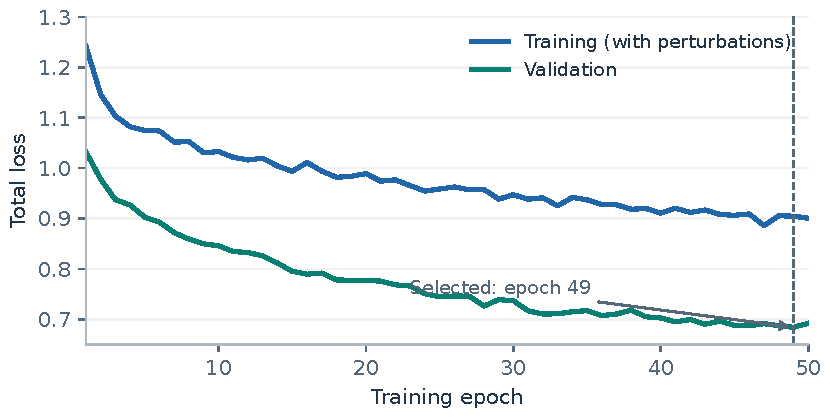
\includegraphics[width=\linewidth]{figures/training_curve.pdf}
\caption{Recorded total training and validation losses. The dashed line identifies the checkpoint selected at epoch 49. These are the weighted objectives in Equation~\eqref{eq:totalloss}, not alignment costs or certificate rates. Training includes dropout and random label remapping; validation does not.}
\label{fig:trainingcurve}
\end{figure}

Replay legality and exact optimality are evaluated outside this differentiable objective. The network learns to imitate aspects of exact solutions; the semantic checks remain explicit computations at use time. This is the reason a poor prediction may reduce candidate quality without invalidating the meaning of a successful replay or an exact certificate.

\section{Implementation and Interactive Use}
\label{sec:implementation}

An alignment method becomes useful to an analyst only when its explanations and evidence can be inspected. This section describes how the mathematical stages are implemented, how the workbench exposes their different outcomes, and how experiments can be reproduced. The interface treats a candidate and its later exact comparison as separate results so that a fast first explanation is never silently presented as an optimum.

\subsection{Software Components and Interfaces}

The implementation is available at \url{https://github.com/fit-alessandro-berti/lara-align}. It uses PyTorch for neural computation and PM4Py for Petri net and event log objects, process discovery, and exact alignment~\cite{Berti2023}. The package provides Python and command line interfaces; the workbench uses Streamlit. Table~\ref{tab:modules} maps the conceptual stages to their implementation modules. This separation allows candidate generation experiments to reuse the same independent verifier.

\begin{table*}[!t]
\caption{Implementation responsibilities in the \texttt{lara\_align} package. A module's output is not given stronger guarantees than the checks it performs.}
\label{tab:modules}
\centering
\begin{tabularx}{\linewidth}{@{}lY@{}}
\toprule
Module & Responsibility\\
\midrule
\texttt{features.py} & Builds typed graph arrays, label IDs, and exact compatibility.\\
\texttt{model.py} & Encodes inputs and returns learned move scores and auxiliary outputs.\\
\texttt{decode.py} & Maintains markings, chooses synchronous transitions, and searches for model move paths.\\
\texttt{verify.py} & Replays complete move sequences, checks projections, and recomputes costs.\\
\texttt{exact.py} & Invokes PM4Py's exact backend and retains concrete transition identities.\\
\texttt{certifier.py} & Exposes proposal and exact comparison operations with explicit statuses.\\
\texttt{families.py}, \texttt{data.py} & Generate behavior families and store inputs, witnesses, and metadata.\\
\texttt{training.py} & Extracts supervision and computes the full training objective.\\
\bottomrule
\end{tabularx}
\end{table*}

An alignment move stores the observed label, transition name, and transition label where applicable. This avoids ambiguity when several transitions share a label. Proposal results retain the candidate, replay report, timings for feature construction/inference/decoding/verification, and optional score diagnostics. Certification results retain the exact witness, exact cost, elapsed time, and status. The candidate is preserved when a better exact alignment becomes available, allowing direct inspection of the gap.

The ordinary alignment entry point supports fast and certified modes. Separate proposal and certification calls support progressive presentation in the workbench. If proposal construction raises an exception, it returns an explicit failure; the workbench can still request exact computation through its separate certification operation. This distinction matters because the convenience alignment call does not automatically recover every possible software failure. The current ``anytime'' mode in the Python enumeration uses the exact comparison path; it is not a learned branch and bound algorithm with a stream of improving lower bounds.

For decoding, the runtime precomputes each transition's preset, postset, label group, and score lookup. Local marking search then operates on sparse token dictionaries and a visited marking set. These implementation choices reduce overhead without changing the firing semantics. Each proposal still constructs its input features and runtime; the reported timing does not assume a globally cached neural representation for a target net. The checkpoint is loaded once before processing a sequence of traces.

\subsection{Preparing a Log and Reference Model}

The Setup page accepts XES event logs, including compressed files, and PNML nets. An analyst may provide an independent reference model or discover a model from the uploaded log using Inductive Miner. The latter option is labeled explicitly: checking a model discovered from the same data is a different analysis from checking compliance with an independently specified process. The discovery noise threshold controls whether infrequent behavior is filtered.

The page summarizes the log and net, lists activity labels and duplicate label groups, and groups cases into variants. Grouping is valid for this control flow setting because cases with the same activity sequence have the same alignment problem against a fixed net and cost policy. It reduces repeated computation while retaining a mapping back to case identifiers. The analyst chooses which variants to process, and the workbench reports the corresponding case coverage. Unprocessed variants are not counted as successful alignments.

\subsection{Progressive Results and Trace Inspection}

The Live Run page offers fast candidates, progressive certification, and an exact baseline. In candidate modes it first produces and independently verifies the proposal for a variant. The result can be displayed immediately, while exact work is a subsequent stage when selected. Statuses distinguish a ready candidate, an illegal candidate, exact computation, certification, repair, timeout, and failure. A timeout retains the evidence already obtained; it does not fill in an unknown optimum.

The Trace Inspector aligns candidate and exact explanations to common observed event positions. It exposes concrete transition identities, which is especially useful for duplicate labels, and allows the model projection to be replayed through precomputed marking snapshots. An analyst can therefore see both where an event was skipped and which enabled transition the decoder chose. Neural score diagnostics are supplementary preferences. They are not labeled as causal explanations or calibrated certainty about correctness.

Results can be exported as variant level and case level CSV, detailed JSON, execution logs, and per alignment move tables. Candidate cost, exact cost, gap, legality, and certification remain separate fields. This makes subsequent analysis auditable: a CSV consumer can select only certified optima or deliberately study the latency and quality of verified candidates. The optional experiment dashboard reads stored metric files for training curve and benchmark inspection.

% Optional insertion point for author supplied screenshots. The scientific
% explanation above is complete without screenshots. See figures/README.md.
\InputIfFileExists{figures/implementation_screenshots.tex}{}{}

\subsection{Reproducibility and Experiment Artifacts}

The journal source includes the reference synthetic corpus, generation configuration, per epoch metrics, and numerical benchmark records. The pretrained checkpoint is distributed separately through the download linked in the Data Availability Statement; its recorded checksum identifies the model used here. The script \texttt{init\_data.py} generates the behavior families; \texttt{train\_model.py} trains and saves checkpoints. Evaluation scripts cover the fixed synthetic test split, scaling inputs, PM4Py approximations, and real logs. The included result data and figure scripts allow the plots to be rebuilt without rerunning training.

Reproducing candidate quality figures requires the recorded checkpoint and matching inputs. Reproducing timings additionally requires the hardware, software, thread settings, and measurement boundaries in Section~\ref{sec:protocol}. Existing result files are measurements of their original runs; rebuilding a plot from those files is not a new runtime experiment. The delivery includes commands for both operations and keeps them separate.

The workbench is an implementation artifact, not a user study result. Its progressive workflow illustrates how to expose the method's guarantees in practice, but the experiments below measure alignment outputs and algorithmic timings. They do not measure analyst productivity, user satisfaction, or deployment performance under concurrent load.

\section{Experimental Evaluation}
\label{sec:evaluation}

The evaluation asks whether the candidate is useful before exact repair and whether machine learning improves that candidate enough to justify its cost. We therefore measure the proposed explanation separately from the exact result. The experiments progress from controlled test families to larger synthetic Petri nets, competing approximations, and real event logs. This order separates the effects of semantic constraints, learned ranking, representation, and input scale.

\subsection{Protocol, Metrics, and Comparison Boundaries}
\label{sec:protocol}

The reference experiments use an Intel Core i7-1355U CPU and the approximately 1.7-million parameter checkpoint selected at epoch 49. Computation is CPU only, with PyTorch reporting ten intra operation and ten inter operation threads; trace calls are sequential. The checkpoint is loaded once before timing. The synthetic test set has 512 rows from 128 generated families, with 64 rows for each motif/representation cell. The scoring parameters stay fixed throughout the test, scaling, and real log experiments.

The primary metrics are replay acceptance, exact cost agreement, and the cost gap in Equation~\eqref{eq:gap}. We also report full transition aware move sequence agreement with the teacher and agreement after replacing transition identities with labels. These sequence measures diagnose imitation of one witness; neither is required for an optimum when several witnesses share its cost. For representation pairs, cost agreement measures whether the same observation receives equal candidate costs on the two equivalent Petri nets.

The guidance ablation preserves the decoder, costs, depth bounds, and test inputs. It disables the neural forward pass and uses deterministic orderings in place of learned rankings. This is a strong baseline because enabledness and bounded model path search already resolve many cases. It directly answers RQ2; comparison with exact search alone would not isolate the contribution of machine learning.

For the LARA timing measurements, fast mode latency includes feature extraction, runtime construction, neural inference when enabled, decoding, and replay. Exact timings include the PM4Py heuristic initialization and search. In the approximation benchmark, the stored timing surrounds the PM4Py alignment call; independent parsing and replay occur afterward. These boundaries are not identical, so small timing differences should not be overinterpreted. All candidate costs are nevertheless compared after replay under the same unit visible deviation policy. Reported medians describe the recorded runs, not a universal hardware independent threshold.

The default test decoder uses catch up depth eight and completion depth 32. Scaling and real log scripts use completion depth 64 while keeping the catch up depth at eight. Exact timeouts in the stress benchmark are 30 seconds, and approximation calls receive five seconds. A timeout leaves the exact cost unknown; the corresponding candidate is included in coverage statistics but excluded from cost gap and optimality calculations that require the optimum. The tables state these denominators explicitly.

For representation specific guidance differences, a family bootstrap constructs 10,000 resampled datasets by drawing whole families with replacement, using seed 13 to make the random draws reproducible. The 2.5th and 97.5th percentiles of the resampled differences define the reported 95\% intervals. A cell contains 32 families with two observations each. Resampling families respects the dependence between observations and representations. These intervals describe sampling within the fixed generator and checkpoint; they do not include variability from retraining with different seeds.

\subsection{Candidate Quality on the Synthetic Test Split}
\label{sec:indist}

The first experiment answers whether the fast pipeline produces complete executable explanations and how close they are to the optimum (RQ1). All 512 candidates pass independent replay. Of these, 466 have the exact optimal cost, giving 91.0\% optimality. Table~\ref{tab:headline} reports the remaining diagnostics and Figure~\ref{fig:gaps} shows the full gap distribution.

\begin{table*}[!t]
\caption{Candidate results on the 512-row synthetic test split. Exact costs come from the teacher/reference alignment; candidate metrics precede any exact repair.}
\label{tab:headline}
\centering
\begin{tabularx}{\linewidth}{@{}Yr@{}}
\toprule
Metric & Result\\
\midrule
Candidate verified by replays & 512/512 (100.0\%)\\
Candidates with optimal cost & 466/512 (91.0\%)\\
Full transition aware move sequence match & 313/512 (61.1\%)\\
Full label level move sequence match & 320/512 (62.5\%)\\
Mean / median cost gap & 0.180 / 0\\
90th / 95th percentile cost gap & 0 / 2\\
Maximum cost gap & 4\\
\bottomrule
\end{tabularx}
\end{table*}

\begin{figure*}[!t]
\centering
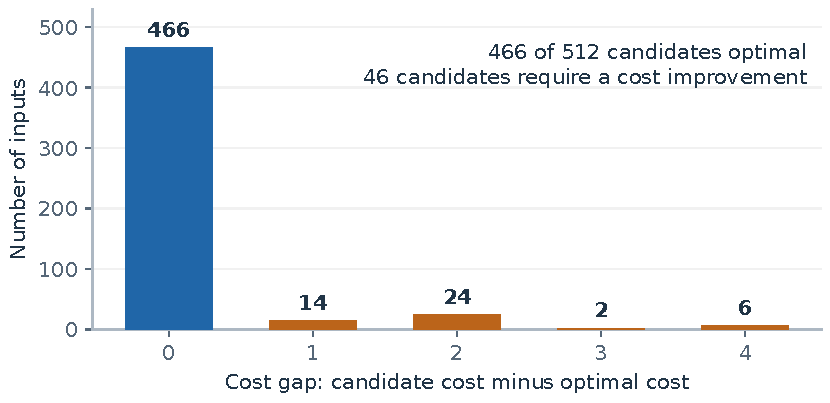
\includegraphics[width=\linewidth]{figures/cost_gaps.pdf}
\caption{All candidate gaps on the test split. Counts sum to 512; 466 candidates have gap zero and 46 have positive gaps. A low mean gap does not make a particular unchecked candidate optimal.}
\label{fig:gaps}
\end{figure*}

The mean gap is small because most candidates are optimal and the remaining gaps are between one and four. Sequence agreement is substantially lower than cost agreement. This is expected when several legal explanations are optimal and the teacher stores one of them. The important distinction for the assurance contract is that replay proves feasibility while exact cost comparison proves optimality, regardless of identity agreement.

When certified mode is evaluated on these inputs, it invokes exact search on all 512. The 466 optimal candidates can be confirmed and retained; the remaining 46 are replaced by exact alignments. The 91.0\% value therefore counts successful proposals, not traces on which exact search was avoided. This experiment establishes useful candidate quality within the generator, while leaving end to end certification acceleration unproven.

\subsection{What Does Learned Guidance Add?}
\label{sec:ablation}

The ablation isolates learned ranking from the model semantics. Unguided decoding also returns 512 legal candidates and reaches optimal cost on 445 of them, or 86.9\%. Adding the learned scorer yields 21 more optimal candidates, an increase of 4.10 percentage points. Mean gap decreases from .258 to .180. Transition aware sequence agreement rises from 57.8\% to 61.1\%, and label level agreement from 58.8\% to 62.5\%.

These aggregate gains are real for the fixed test set but do not imply that machine learning is responsible for most successful alignments. The unguided decoder already synchronizes uniquely enabled matches and searches for short model move paths. Many inputs offer little meaningful ranking choice. To answer where the improvement comes from, Table~\ref{tab:classes} separates the eight representation cells and Figure~\ref{fig:guidance} shows the corresponding differences.

\begin{table*}[!t]
\caption{Optimality by motif and representation. Each cell contains 64 inputs. G and U identify guided and unguided decoding; all outputs pass replay. Mean gaps are reported for guided candidates.}
\label{tab:classes}
\centering
\begin{tabularx}{\linewidth}{@{}lYrrr@{}}
\toprule
Motif & Representation & G optimal & U optimal & G mean gap\\
\midrule
Ordinary tree & Canonical block & 54/64 (84.4\%) & 55/64 (85.9\%) & .344\\
Ordinary tree & Isomorphic rename & 54/64 (84.4\%) & 49/64 (76.6\%) & .344\\
Duplicate/silent & Duplicate prefix & 61/64 (95.3\%) & 44/64 (68.8\%) & .094\\
Duplicate/silent & Silent routing & 63/64 (98.4\%) & 63/64 (98.4\%) & .031\\
Concurrency & Parallel & 58/64 (90.6\%) & 58/64 (90.6\%) & .219\\
Concurrency & Interleaving & 58/64 (90.6\%) & 58/64 (90.6\%) & .219\\
M pattern & Canonical block & 59/64 (92.2\%) & 59/64 (92.2\%) & .094\\
M pattern & Non-free choice & 59/64 (92.2\%) & 59/64 (92.2\%) & .094\\
\bottomrule
\end{tabularx}
\end{table*}

\begin{figure*}[!t]
\centering
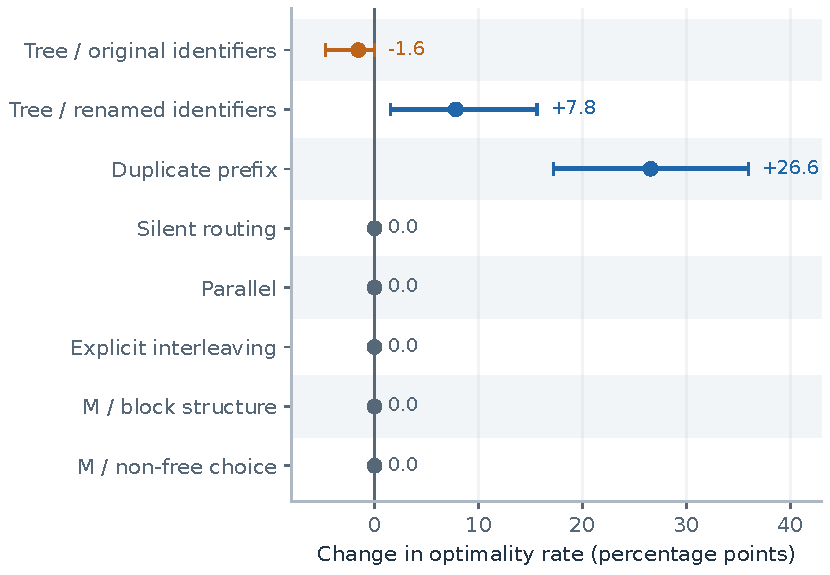
\includegraphics[width=\linewidth]{figures/guidance_effect.pdf}
\caption{Change in optimality rate when the fixed scorer is enabled. Positive values favor guidance. Intervals are 95\% percentile intervals from 10,000 family level bootstrap resamples; the zero width intervals indicate identical sampled success differences, not certainty about other generators. The strongest gain is concentrated in duplicate prefix choices.}
\label{fig:guidance}
\end{figure*}

The duplicate prefix cell improves from 68.8\% to 95.3\%, a gain of 26.6 points, with a family bootstrap interval of $[17.2,35.9]$ points. This is the case in which the trace suffix can distinguish two currently enabled transitions with the same label. Silent routing already attains 98.4\% without machine learning: its bounded search can postpone the choice until the distinguishing event. Guided and unguided costs coincide on the parallel/interleaving and M cells. RQ2 therefore has a localized answer: the measured gain is strongest where the decoder must commit before structural enabledness resolves the ambiguity.

\subsection{Sensitivity to Equivalent Representations}
\label{sec:representations}

Equivalent models let us examine reuse without changing the visible alignment problem (RQ3). Table~\ref{tab:pairagreement} compares candidate costs across each representation pair for the same observation. The ordinary tree pair is particularly informative because the two Petri nets differ only in identifiers.

\begin{table*}[!t]
\caption{Candidate cost agreement across paired representations. Each row compares 64 observation pairs. Exact costs agree in every pair. Candidate cost equality may include two equally suboptimal results.}
\label{tab:pairagreement}
\centering
\begin{tabularx}{\linewidth}{@{}Yrr@{}}
\toprule
Equivalent representation pair & Guided agreement & Unguided agreement\\
\midrule
Canonical tree / isomorphic rename & 100.0\% & 90.6\%\\
Duplicate prefix / silent routing & 96.9\% & 70.3\%\\
Parallel / explicit interleaving & 100.0\% & 100.0\%\\
Block M / non-free-choice M & 100.0\% & 100.0\%\\
\midrule
All 256 observation pairs & 99.2\% & 90.2\%\\
\bottomrule
\end{tabularx}
\end{table*}

Guided decoding reaches 84.4\% optimality on both canonical and renamed trees, with identical paired costs. Unguided decoding falls from 85.9\% to 76.6\% after renaming. Guidance is thus slightly worse on canonical identifiers, by $-1.6$ points with interval $[-4.7,0.0]$, but better on the renamed identifiers by $+7.8$ points with interval $[1.6,15.6]$. These signs have a common explanation: deterministic name order happens to be favorable on one numbering and less favorable on the other. The learned scorer maintains the same quality across this tested renaming.

Across all representation pairs, agreement rises from 90.2\% to 99.2\%. This is evidence of stability for the tested transformations, not proof of invariance under every isomorphism or activity relabeling. Ties, numerical behavior, and changed label embeddings can still affect choices. It also does not establish transfer to unseen compilation schemes: all four representation families occur during training.

\subsection{Scaling: Candidate Latency and Quality Together}
\label{sec:scaling}

The scaling experiment tests whether the candidate remains useful when inputs move beyond the small training distribution. A separate generator produces random block structured Petri nets with sequence, choice, parallelism, loops, duplicate labels, and invisible routing. The nominal sizes are 5, 10, 20, and 40 visible leaf occurrences. An alphabet fraction of .7 permits repeated labels; loop playout uses redo probability .3 and at most two redos. Deviations are injected at rates .15 and .35, with ten inputs per configuration. These rates are parameters of the stress generator, not the clean/noisy mixture in Section~\ref{sec:corruption}. Table~\ref{tab:scaling} reports the sizes, quality measures, and timings for all eight configurations.

\begin{table*}[!t]
\caption{Scaling results. Size is the requested visible leaf count and $\overline{|T|}$ the rounded mean total transition count. Every configuration has ten legal candidates. $n_\delta$ is the number with an exact reference; optimality and mean gap use that denominator. Time columns are median milliseconds per trace; exact timeouts are recorded at 30 seconds.}
\label{tab:scaling}
\centering
\begin{tabular}{@{}rrrrrrrr@{}}
\toprule
Size & Deviation & $\overline{|T|}$ & $n_\delta$ & Optimal & Mean gap & Fast ms & Exact ms\\
\midrule
5 & .15 & 7 & 10 & 90.0\% & .2 & 5.5 & 1.3\\
5 & .35 & 6 & 10 & 60.0\% & 1.6 & 4.6 & 1.3\\
10 & .15 & 13 & 10 & 80.0\% & 1.2 & 5.0 & 1.8\\
10 & .35 & 13 & 10 & 50.0\% & 1.7 & 5.3 & 2.8\\
20 & .15 & 28 & 10 & 60.0\% & 3.6 & 6.9 & 2.9\\
20 & .35 & 26 & 10 & 60.0\% & 3.1 & 6.0 & 11.7\\
40 & .15 & 55 & 10 & 30.0\% & 8.1 & 8.7 & 63.9\\
40 & .35 & 54 & 9 & 44.4\% & 11.7 & 8.6 & 24.7\\
\bottomrule
\end{tabular}
\end{table*}

\begin{figure*}[!t]
\centering
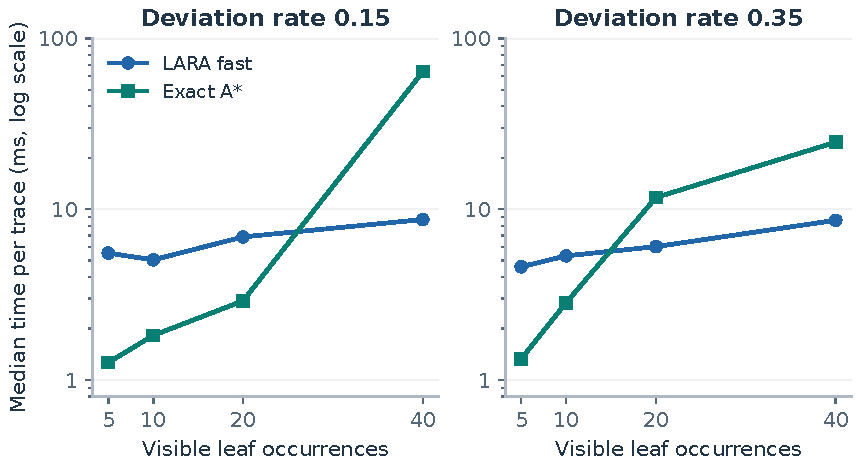
\includegraphics[width=\linewidth]{figures/scaling_latency.pdf}
\caption{Recorded median latencies on the scaling grid. The vertical axis is logarithmic; the horizontal axis is the number of visible leaf occurrences, not distinct activity labels. Exact search is faster on smaller cells, while its median is larger on several larger cells. These observations do not establish an asymptotic runtime law.}
\label{fig:scalingtime}
\end{figure*}

Figure~\ref{fig:scalingtime} compares the median latencies across this grid. LARA's guided median ranges from 4.6 to 8.7 ms. Exact A* is faster on the small configurations. It becomes slower at size 20 with deviation .35, and at size 40 for both rates. At size 40 and deviation .15 the median ratio is approximately $63.9/8.7=7.34$ in favor of the fast candidate. One exact call times out at size 40 and deviation .35. These are candidate latency comparisons, not certified mode speedups.

\begin{figure*}[!t]
\centering
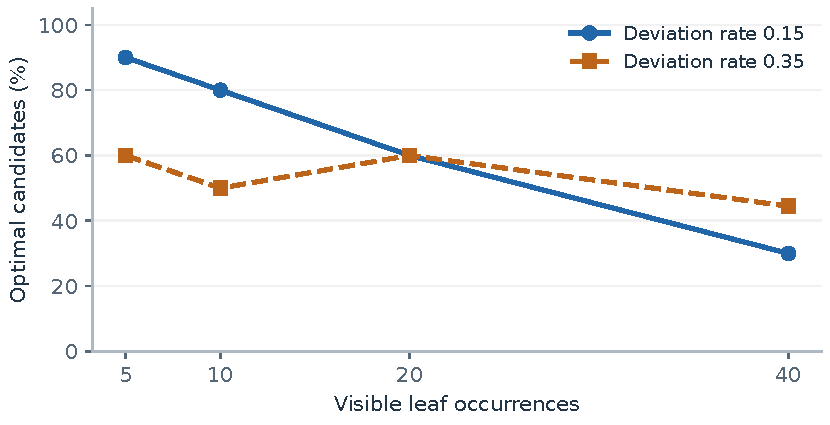
\includegraphics[width=\linewidth]{figures/scaling_quality.pdf}
\caption{The quality cost of the latency advantage in Figure~\ref{fig:scalingtime}. Optimality declines on larger stress inputs. Each point uses ten exact references except size 40/deviation .35, which uses nine. Small cell sizes and changing random Petri nets explain why the curves need not be monotone.}
\label{fig:scalingquality}
\end{figure*}

Figure~\ref{fig:scalingquality} shows the accompanying decline in quality: at size 40 only 30.0\% or 44.4\% of comparable candidates are optimal, and mean gaps reach 8.1 or 11.7. Replay remains successful on all 80 candidates, demonstrating executability despite this loss of quality. Unguided decoding takes approximately .2--1.2 ms across the grid and is faster than the exact medians throughout. Guidance contributes little on this stress distribution. The practical question is therefore whether better rankings justify the neural inference cost, not simply whether a neural forward pass is faster than a difficult exact search.

\subsection{Comparison with Established Approximations}
\label{sec:approximations}

Competing candidate generators provide a more demanding test than exact search alone. The benchmark uses PM4Py 2.7.23.2 implementations of discounted A*~\cite{Boltenhagen2021}, tandem repeats~\cite{ReissnerTandem2020}, sliding windows~\cite{Bogdanov2024}, fixed horizon search~\cite{Dongen2017}, and subset/edit distance approximation~\cite{FaniSani2020}. Sliding windows use length 20 and at most five candidates; the fixed horizon is four; the configured expansion budget is 100,000 where supported. The subset size is one within each model variant group and is evaluated only on the test corpus. These are concrete settings, not tuned best case envelopes for each method.

All returned alignments are parsed into transition aware moves, replayed independently, and rescored with the same costs. This is particularly important for discounted objectives: their internally reported objective need not equal the ordinary visible deviation count. Table~\ref{tab:approxsmall} reports the test comparison, and Table~\ref{tab:approxstress} reports stress results from the approximation benchmark run.

\begin{table*}[!t]
\caption{Candidate quality on the synthetic test split. All six methods provide 512 legal outputs in this experiment, so the optimality denominator is 512 for every row.}
\label{tab:approxsmall}
\centering
\begin{tabularx}{\linewidth}{@{}Yrr@{}}
\toprule
Method & Optimal candidates & Mean gap\\
\midrule
LARA guided & 466/512 (91.0\%) & .180\\
Discounted A* & 490/512 (95.7\%) & .090\\
Tandem repeats & 502/512 (98.0\%) & .039\\
Sliding window & 512/512 (100.0\%) & .000\\
Fixed horizon & 502/512 (98.0\%) & .047\\
Subset/edit distance & 360/512 (70.3\%) & .637\\
\bottomrule
\end{tabularx}
\end{table*}

Every tested Petri net search/compression approximation exceeds LARA's optimality rate on the small corpus. LARA exceeds the particular subset/edit distance configuration. All test traces fit within one sliding window of 20 events, so the perfect result in that row does not exercise the approximation caused by crossing a window boundary. The comparison illustrates why a small benchmark can be useful for diagnosis without being a sufficient stress test.

\begin{table*}[!t]
\caption{Stress comparison over 80 inputs. Coverage counts legal outputs out of all 80; $n_\delta$ counts legal outputs with an exact reference. Optimality and mean gap are conditional on those $n_\delta$ inputs. Time is the median over all calls, including unsuccessful calls. Different coverage denominators limit direct quality comparisons.}
\label{tab:approxstress}
\centering
\begin{tabularx}{\linewidth}{@{}Yrrrrr@{}}
\toprule
Method & Coverage & $n_\delta$ & Optimal & Mean gap & Median ms\\
\midrule
LARA guided & 80/80 & 79 & 59.5\% & 3.797 & 7.69\\
Discounted A* & 80/80 & 79 & 75.9\% & 1.468 & 1.17\\
Tandem repeats & 78/80 & 78 & 93.6\% & .128 & 1.37\\
Sliding window & 79/80 & 79 & 100.0\% & .000 & 1.27\\
Fixed horizon & 76/80 & 76 & 82.9\% & 2.263 & 82.37\\
\bottomrule
\end{tabularx}
\end{table*}

The stress comparison again favors established approximations in quality. Discounted A* has the same full legal coverage as LARA, a higher exact cost rate, a smaller mean gap, and a lower recorded median latency. Tandem repeats and sliding windows are even closer to optimal where they return comparable results. Their incomplete coverage must remain visible: a perfect conditional optimum rate is not a result on every attempted input. LARA's full coverage is useful, but it is not unique to the learned method on this grid.

The small and stress comparisons rule out a claim that the present learned greedy decoder is the best general approximation. They instead identify a reusable scoring mechanism with a measured local advantage over its own unguided baseline. Any later claim of competitive overall approximation quality requires a stronger decoder and renewed comparison using common timing boundaries and coverage accounting.

\subsection{Application to Public Event Logs without Fine Tuning}
\label{sec:real}

Real log inputs test the use of one checkpoint with different vocabularies, model structures, and trace lengths. We use a building permit receipt log~\cite{ReceiptLog}, containing 1434 cases, 116 variants, and 27 activity labels, and the repository's 100-case sample of the road traffic fines log~\cite{RoadTrafficLog}, containing ten variants and ten labels. The road traffic results refer to that sample, not the complete public log. The longest variants have 25 and nine events, respectively.

For each log, PM4Py discovers Petri nets using Inductive Miner~\cite{Leemans2013} at noise threshold .0 and its infrequent behavior variant~\cite{Leemans2014} at threshold .5. Models are discovered from the same log that is subsequently aligned, so this experiment evaluates algorithmic transfer, not independent normative compliance. The positive noise threshold removes infrequent behavior and creates additional deviations against the resulting model. The checkpoint is unchanged; new label strings enter through hashing without any language interpretation or fine tuning.

\begin{table*}[!t]
\caption{Real log candidate quality. All variants pass replay. Petri net size gives places and visible/invisible transitions. Guided and unguided decoding have identical quality values in all four configurations. Mean and maximum gaps are over variants.}
\label{tab:realquality}
\centering
\begin{tabular}{@{}llrrrr@{}}
\toprule
Log & Noise & Petri net size & \multicolumn{2}{c}{Optimal (\%)} & Gap\\
 & & $|P|/|T_v|+|T_\tau|$ & Variants & Cases & Mean/max\\
\midrule
Road traffic & .0 & $15/10+10$ & 100.0\% & 100.0\% & 0/0\\
Road traffic & .5 & $13/10+7$ & 70.0\% & 94.0\% & .50/3\\
Receipt & .0 & $45/27+47$ & 50.0\% & 82.6\% & .76/5\\
Receipt & .5 & $25/24+19$ & 55.2\% & 74.6\% & .82/7\\
\bottomrule
\end{tabular}
\end{table*}

Table~\ref{tab:realquality} distinguishes variants from cases. If variant $v$ occurs $f_v$ times, case weighted optimality is
\begin{equation}
 \frac{\sum_v f_v\ind[g_v=0]}{\sum_vf_v},
 \label{eq:weighted}
\end{equation}
whereas variant optimality weights each distinct sequence once. The higher case weighted values show that frequent variants are easier for this decoder; misses are concentrated in less frequent variants. For the fitting receipt Petri net, all exact costs are zero, but only half of the candidate variants attain zero. A legal, positive cost candidate on a fitting trace is therefore a concrete example of why replay alone is insufficient to infer nonconformance.

\begin{table*}[!t]
\caption{Recorded median time per variant in milliseconds. These are candidate/exact timings, not full log wall clock speedups. Including the unguided decoder makes clear that the real log candidate advantage is not evidence of a learned quality benefit.}
\label{tab:realtime}
\centering
\begin{tabularx}{\linewidth}{@{}Yrrrr@{}}
\toprule
Log & Noise & Guided fast & Unguided fast & Exact A*\\
\midrule
Road traffic & .0 & 5.39 & .56 & 1.92\\
Road traffic & .5 & 5.22 & .48 & 1.56\\
Receipt & .0 & 16.05 & 6.01 & 31.04\\
Receipt & .5 & 6.65 & .61 & 12.72\\
\bottomrule
\end{tabularx}
\end{table*}

The guided candidate is slower than exact search on the small road traffic Petri nets and faster on the tested receipt Petri nets (Table~\ref{tab:realtime}). Unguided decoding is faster still and has the same candidate quality. These discovered Petri nets have no duplicate visible labels, so they do not exercise the scorer's strongest demonstrated advantage. Model move ordering could still matter in principle, but no quality difference is observed here. The experiment supports interface transfer and verified execution under different inputs; it does not demonstrate that the neural scorer improves real log alignment quality.

\subsection{A Failure That Explains the Remaining Gaps}
\label{sec:failure}

Aggregate rates show how often the decoder fails to be optimal; the worked failure in Figure~\ref{fig:failure} explains why. Consider test observation $\langle A,D,B,C,C,D\rangle$ in the parallel/interleaving family. Its process permits $A,B$ in either order, then $C,D$. An optimal alignment skips the early $D$ and one repeated $C$, giving cost two. LARA instead inserts model moves $B,C$ so that it can synchronize the early $D$. It reaches the final marking while four observed events remain, forcing four log moves. Its total cost is six, hence gap four.

\begin{figure*}[!t]
\centering
\begin{tikzpicture}[x=1cm,y=1cm]
\node[paneltitle] at (0,.95) {A. Skip the early $D$ and one repeated $C$};
\node[annotation,anchor=east] at (1,0) {log};
\node[annotation,anchor=east] at (1,-.7) {model};
\foreach \x/\l/\m in {1.7/A/A,3.9/B/B,5/C/C,7.2/D/D}{
\node[alcell] at (\x,0) {$\l$};\node[alcell] at (\x,-.7) {$\m$};}
\foreach \x/\l in {2.8/D,6.1/C}{
\node[devcell] at (\x,0) {$\l$};\node[devcell] at (\x,-.7) {$\skipmove$};}
\node[verifybox,text width=16mm] at (9.35,-.35) {optimal\\cost $2$};
\node[annotation,anchor=west] at (1.15,-1.4) {4 synchronous moves + 2 log moves};
\node[paneltitle] at (0,-2.35) {B. Catch up to the early $D$, then finish too soon};
\node[annotation,anchor=east] at (1,-3.3) {log};
\node[annotation,anchor=east] at (1,-4) {model};
\foreach \x/\l/\m in {1.7/A/A,5/D/D}{
\node[alcell,fill=softblue] at (\x,-3.3) {$\l$};\node[alcell,fill=softblue] at (\x,-4) {$\m$};}
\foreach \x/\m in {2.8/B,3.9/C}{
\node[devcell] at (\x,-3.3) {$\skipmove$};\node[devcell] at (\x,-4) {$\m$};}
\foreach \x/\l in {6.1/B,7.2/C,8.3/C,9.4/D}{
\node[devcell] at (\x,-3.3) {$\l$};\node[devcell] at (\x,-4) {$\skipmove$};}
\draw[devamber,line width=1pt] (2.25,-4.55) -- (4.45,-4.55);
\draw[devamber,line width=1pt] (5.55,-4.55) -- (9.95,-4.55);
\node[annotation,text=devamber] at (3.35,-4.95) {2 model moves};
\node[annotation,text=devamber] at (7.75,-4.95) {4 log moves after completion};
\node[warnbox,text width=100mm] at (5.5,-6) {Candidate cost $2+4=6$; optimal cost $2$; gap $4$.\\Every firing is legal, but the early decision harms the suffix.};
\end{tikzpicture}

\caption{A legal but suboptimal explanation of $\langle A,D,B,C,C,D\rangle$. Each visible deviation is amber. Invisible routing is omitted, and model rows display activity labels for readability. The upper explanation costs two; the lower costs six. The early attempt to synchronize $D$ causes both the two inserted model activities and the four subsequent skipped events.}
\label{fig:failure}
\end{figure*}

The error is a decoder commitment, not a replay failure. The decoder tries a bounded model path before considering a log move and never compares that path with skipping the early $D$. The trained log score is unused, and earlier choices cannot be revised. Better duplicate label scoring cannot fix every instance of this mechanism. It motivates joint ranking of synchronous, log, and model alternatives and retaining several candidate continuations, as discussed next.

\section{Discussion and Limitations}
\label{sec:discussion}

The results are most useful when they guide a concrete choice about when to generate a candidate and what to infer from it. This section connects the three research questions to that choice, distinguishes the semantic contract from empirical performance, and identifies the changes needed for stronger claims. It also records limits of the evidence so that the observed transfer is not mistaken for general-purpose alignment competence.

\subsection{Interpreting the Three Research Questions}

For RQ1, the experiments show that the decoder and replay pipeline produced legal candidates on all evaluated inputs, with 91.0\% optimality on the controlled test split. The formal guarantee is conditional: when replay accepts, the candidate is a complete executable explanation and its cost is an upper bound. The observed 100\% acceptance rate does not prove that the bounded decoder always reaches the final marking. Larger gaps on stress inputs and the worked failure show that a reliable legality check can coexist with a weak candidate policy.

For RQ2, learning has a measurable but concentrated effect. The duplicate-prefix improvement demonstrates that global trace context can help decide among equal labels before the decoder reaches their distinguishing continuation. The identifier-renaming experiment shows more stable candidate costs than the name-ordered baseline. The remaining motifs show no cost improvement. The evidence therefore supports using learned rankings for selected ambiguities, rather than attributing the overall success rate to the network.

For RQ3, one checkpoint accepts new net sizes and label vocabularies without fine tuning. The candidate can arrive faster than the tested exact backend on larger receipt models and selected stress cells. However, guided inference imposes a substantial floor on small cases, quality degrades on larger stress inputs, and established approximations perform better overall. The real-log quality is identical without learning. Reuse is demonstrated at the interface and candidate-pipeline level, while broad learned generalization remains limited.

\subsection{What a Verified Candidate Can and Cannot Tell an Analyst}

A verified candidate is useful because it is an executable explanation of the observed case. It can support visualization, an initial inspection of deviations, and a bound on the best achievable cost. Its deviation locations should nevertheless be read in the light of its optimization status. The fitting receipt model makes this concrete: a positive candidate cost does not prove that the trace deviates from the model, because a zero-cost alignment may exist. If the goal is to assert the minimum deviation count, exact evidence remains necessary.

Likewise, equal optimal costs do not identify a unique diagnostic story. Different optimal alignments may allocate deviations or synchronize independent activities differently. Certification establishes minimal cost under the chosen policy, not the uniquely correct account of what happened in the organization. Business interpretation still depends on the model, event-data quality, and the suitability of the cost function.

Progressive presentation is a practical application of these distinctions. A workbench can show a candidate and its replay status immediately, then add exact comparison when available. The current implementation supports that sequence. A deployment policy that starts exact search first and invokes candidate generation only for slow cases could reduce unnecessary inference, but this policy has not been evaluated. The threshold would depend on model structure, hardware, expected quality, and the analyst's need for a certificate.

\subsection{Threats to Validity}
\label{sec:validity}

\textbf{Training distribution.} The corpus is small and intentionally structured. It contains four motif types, three of which use fixed controlled constructions. Family-level splitting prevents separation of a generated family's views, but it does not exclude repeated visible languages or motifs across splits. Holding out whole motif classes, unseen compilation schemes, or larger and more varied net collections would provide stronger evidence of structural transfer. Training on abstract labels also leaves business semantics, resources, and time outside the study.

\textbf{Teacher and objective.} Exact targets are verified for the supplied cost model, but only one optimal witness is retained. Sequence agreement therefore mixes candidate quality with witness choice. The masking rule for duplicate-prefix targets is motif-specific. Moreover, the loss supervises a log head that decoding ignores and auxiliary region heads whose contribution has not been isolated. These choices make the trained model a useful experimental prototype, but they do not establish that the objective is the best one for candidate cost.

\textbf{Statistical coverage.} The main result uses one checkpoint and one training seed. Bootstrap intervals resample families for that fixed model; they are not intervals over retraining or target domains. Stress cells contain only ten inputs, and the real-log study uses two logs with one restricted road-traffic sample. Observed perfect coverage or agreement in these collections should not be generalized to arbitrary systems.

\textbf{Comparison protocol.} The evaluation uses one exact backend and concrete approximation configurations. Alternatives such as stronger exact implementations, other window sizes, or larger representative subsets may change the comparison. Stored PM4Py approximation times exclude the independent wrapper replay, whereas LARA proposal timing includes it. Hardware scheduling, warm-up effects, and Python overhead can affect millisecond-scale differences. The strongest present comparative evidence concerns the replayed costs and explicit coverage; fine-grained timing claims require a common harness and repeated measurements.

\textbf{Real-log interpretation.} Models are discovered from the same logs used for alignment. This is appropriate for testing the algorithm on different structures and labels, but it does not establish compliance with an independent organizational specification. Variant and case weighting answer different questions, and selecting a limited set of variants in an interactive run changes the covered population. The paper therefore reports both quality weightings and states the scope of the road-traffic sample.

\textbf{Semantic and computational scope.} The evaluated setting uses ordinary control-flow nets and fixed unit visible-deviation costs. Neural features omit explicit arc weights, current decoder markings, and data guards. The scorer uses dense attention, and the decoder's depth bounds do not bound the width of marking exploration. Neither component has a demonstrated constant-latency guarantee. The guarantee that survives these implementation limits is the conditional replay/certification contract.

\subsection{Methodological Extensions Suggested by the Evidence}

The failure in Figure~\ref{fig:failure} suggests comparing a log move with model catch-up before committing. A decoder could rank synchronous, log, and model alternatives jointly and retain a small beam of partial alignments. Recomputing scores from the current marking or predicting model preferences per event position could help it respond to earlier choices. These changes would increase inference or search cost, so they should be assessed against both the current unguided decoder and strong non-neural approximations.

A separate extension concerns certification. A replay-verified candidate supplies a feasible incumbent cost. An exact search algorithm can potentially use that cost for pruning while relying on admissible lower bounds for correctness. Such an integration would need to expose the relevant solver interface, preserve exactness, and demonstrate reduced total work. Merely comparing a candidate with an independently computed optimum, as done here, cannot support a certification-speedup claim.

Training could also focus on the decisions that the active decoder actually makes, collect multiple optimal witnesses, or penalize downstream candidate gaps more directly. Additional structural diversity and deliberate tests of hash relabeling would strengthen evidence for reuse. The auxiliary regions would require independent validation before being treated as meaningful process decompositions. These are research directions motivated by observed limitations, not capabilities of the evaluated checkpoint.

\section{Conclusions}
\label{sec:conclusion}

The aim of this study is to determine a useful role for reusable learning in alignment-based conformance checking while keeping the meaning of an explanation explicit. LARA combines a pretrained graph-and-trace scorer with a marking-aware decoder, independent replay, and optional exact comparison. The scorer proposes move preferences; replay establishes executability and an upper bound; successful exact computation establishes the optimum or supplies a replacement.

On the controlled synthetic test set, guidance increases optimal candidates from 445 to 466 out of 512, with its largest contribution on duplicate-prefix choices. All evaluated candidates pass replay, but candidate quality falls on larger stress inputs. Real-log experiments show that the fixed checkpoint can be used with new vocabularies and model structures, while providing no quality improvement over the unguided decoder on those logs. Established approximations generally perform better in the direct comparisons, and the current certified mode still runs exact search for every trace.

The resulting contribution is a transparent, reproducible study of learned candidate scoring within an alignment pipeline whose guarantees come from process semantics. The most promising next steps are stronger decisions among competing move types, broader tests of structural transfer, and using verified incumbents to reduce exact search work. Their value must be demonstrated in candidate quality and total computation, with the same explicit separation between a plausible prediction and a proven alignment property.

\authorcontributions{Software, A.B.; writing---review and editing, A.B. and W.M.P.v.d.A.}
\funding{Funded by the European Union. This work has received funding from the European High Performance Computing Joint Undertaking (JU) and from the German Federal Ministry of Research, Technology and Space (BMFTR), the Ministry of Culture and Science of North Rhine-Westphalia (MKW NRW), and the Hessian Ministry of Science and Research, Arts and Culture (HMWK) under grant agreement No.~101250682.}
\institutionalreview{Not applicable. This study uses synthetic traces and previously published event logs.}
\informedconsent{Not applicable.}
\dataavailability{The application is publicly available at \url{https://lara-pm.app}. The implementation and experiment scripts are available at \url{https://github.com/fit-alessandro-berti/lara-align}. The \texttt{ft-journal} branch includes the reference synthetic corpus, numerical result records, and figure sources in \texttt{paper\_applsci}. The pretrained checkpoint is available at \url{https://www.alessandroberti.it/checkpoint_lara_latest.tar.gz}; the journal source records its SHA-256 checksum. A footnote in Section~\ref{sec:implementation} provides both data and trained checkpoint download links. The public event log sources are cited in Section~\ref{sec:real}.}
\acknowledgments{Generative AI tools (OpenAI Codex) supported software implementation and manuscript generation. The authors take responsibility for the content.}
\conflictsofinterest{W.M.P.v.d.A. is affiliated with Celonis.}
\abbreviations{Abbreviations}{The following abbreviations are used in this manuscript:\\
\begin{tabular}{@{}ll}
A* & Heuristic shortest path search\\
BFS & Breadth first search\\
CPU & Central processing unit\\
GNN & Graph neural network\\
LARA & Learned Alignment with Replay Assurance\\
PNML & Petri Net Markup Language\\
RQ & Research question\\
XES & eXtensible Event Stream
\end{tabular}}
\reftitle{References}
\bibliography{references}
\end{document}
